%%%%%%%%%%%%%%%%%%%%%%%%%%%%%%%%%%%%%%%%%%%%%%%
%
% Template per Elaborato di Laurea
% DISI - Dipartimento di Ingegneria e Scienza dell’Informazione
%
% update 2015-09-10
%
% Per la generazione corretta del 
% pdflatex nome_file.tex
% bibtex nome_file.aux
% pdflatex nome_file.tex
% pdflatex nome_file.tex
%
%%%%%%%%%%%%%%%%%%%%%%%%%%%%%%%%%%%%%%%%%%%%%%%

% formato FRONTE RETRO
\documentclass[epsfig,a4paper,11pt,titlepage,twoside,openany]{book}
\usepackage{epsfig}
\usepackage{plain}
\usepackage{setspace}
\usepackage[paperheight=29.7cm,paperwidth=21cm,outer=1.5cm,inner=2.5cm,top=2cm,bottom=2cm]{geometry} % per definizione layout
\usepackage{titlesec} % per formato custom dei titoli dei capitoli

%%%%%%%%%%%%%%
% supporto lettere accentate
%
%\usepackage[latin1]{inputenc} % per Windows;
\usepackage[utf8x]{inputenc} % per Linux (richiede il pacchetto unicode);
%\usepackage[applemac]{inputenc} % per Mac.

\singlespacing

\usepackage[italian]{babel}

\begin{document}

  % nessuna numerazione
  \pagenumbering{gobble} 
  \pagestyle{plain}

\thispagestyle{empty}

\begin{center}
  \begin{figure}[h!]
    \centerline{
\psfig{file=logo_unitn_black_center.png,width=0.6\textwidth}}
  \end{figure}

  \vspace{2 cm} 

  \LARGE{Dipartimento di Ingegneria e Scienza dell’Informazione\\}

  \vspace{1 cm} 
  \Large{Corso di Laurea in\\
    ...
    %Informatica
    %Ingegneria dell'Informazione e delle Comunicazioni
    %Ingegneria dell'Informazione e Organizzazione d'Impresa
    %Ingegneria Elettronica e delle Telecomunicazioni
  }

  \vspace{2 cm} 
  \Large\textsc{Elaborato finale\\} 
  \vspace{1 cm} 
  \Huge\textsc{Titolo\\}
  \Large{\it{Sottotitolo (alcune volte lungo - opzionale)}}


  \vspace{2 cm} 
  \begin{tabular*}{\textwidth}{ c @{\extracolsep{\fill}} c }
  \Large{Supervisore} & \Large{Laureando}\\
  \Large{......}& \Large{......}\\
  \end{tabular*}

  \vspace{2 cm} 

  \Large{Anno accademico .../...}
  
\end{center}



  \clearpage
 
%%%%%%%%%%%%%%%%%%%%%%%%%%%%%%%%%%%%%%%%%%%%%%%%%%%%%%%%%%%%%%%%%%%%%%%%%%
%%%%%%%%%%%%%%%%%%%%%%%%%%%%%%%%%%%%%%%%%%%%%%%%%%%%%%%%%%%%%%%%%%%%%%%%%%
%% Nota
%%%%%%%%%%%%%%%%%%%%%%%%%%%%%%%%%%%%%%%%%%%%%%%%%%%%%%%%%%%%%%%%%%%%%%%%%%
%% Sezione Ringraziamenti opzionale
%%%%%%%%%%%%%%%%%%%%%%%%%%%%%%%%%%%%%%%%%%%%%%%%%%%%%%%%%%%%%%%%%%%%%%%%%%
%%%%%%%%%%%%%%%%%%%%%%%%%%%%%%%%%%%%%%%%%%%%%%%%%%%%%%%%%%%%%%%%%%%%%%%%%%
  \thispagestyle{empty}

\begin{center}
  {\bf \Huge Ringraziamenti}
\end{center}

\vspace{4cm}


\emph{
  Ringrazio innanzitutto Farnedi ICT per avermi permesso di basare la mia tesi su questo progetto e avermi concesso il tempo e le risorse per dedicarmi alla creazione di questo elaborato.}	\vspace{5mm}
  
  \emph{
  Ringrazio il professor Marchese per avermi indirizzato e seguito nella stesura di questa tesi.}	\vspace{5mm}
  
  \emph{
 Ringrazio la mia famiglia che mi ha sostenuto e dato consiglio}	\vspace{5mm}
 
  \emph{
 Ringrazio mia madre più di tutti perché mi ha sempre spronato a dare il massimo e non scendere a compromessi. Ringrazio mio padre che, a modo suo, mi ha passato la passione per questo splendido mondo e mestiere}	\vspace{5mm}
 
 \emph{
 Ringrazio Leonardo Herzog, Alessandro Olivo, Jacopo Oss Eberle, Filippo Festini e Andrea Sosi per avermi dato sostegno nel momento in cui ne avevo più bisogno}	\vspace{5mm}
 
 \emph{
  Ringrazio Greta che, durante questo viaggio, mi è sempre stata vicina e mi ha sempre indicato la giusta via.}	\vspace{5mm}

  \clearpage
  \pagestyle{plain} % nessuna intestazione e pie pagina con numero al centro

  
  % inizio numerazione pagine in numeri arabi
  \mainmatter

%%%%%%%%%%%%%%%%%%%%%%%%%%%%%%%%%%%%%%%%%%%%%%%%%%%%%%%%%%%%%%%%%%%%%%%%%%
%%%%%%%%%%%%%%%%%%%%%%%%%%%%%%%%%%%%%%%%%%%%%%%%%%%%%%%%%%%%%%%%%%%%%%%%%%
%% Nota
%%%%%%%%%%%%%%%%%%%%%%%%%%%%%%%%%%%%%%%%%%%%%%%%%%%%%%%%%%%%%%%%%%%%%%%%%%
%% Si ricorda che il numero massimo di facciate e' 30.
%% Nel conteggio delle facciate sono incluse 
%%   indice
%%   sommario
%%   capitoli
%% Dal conteggio delle facciate sono escluse
%%   frontespizio
%%   ringraziamenti
%%   allegati    
%%%%%%%%%%%%%%%%%%%%%%%%%%%%%%%%%%%%%%%%%%%%%%%%%%%%%%%%%%%%%%%%%%%%%%%%%%
%%%%%%%%%%%%%%%%%%%%%%%%%%%%%%%%%%%%%%%%%%%%%%%%%%%%%%%%%%%%%%%%%%%%%%%%%%

    % indice
    \tableofcontents
    \clearpage
    
 %%%%%%%%%%%%%%%%%%%%%%%%%%%%%%%%%%%%%%%%%%%%%%%%%%%%%%%%%%%%%%%%%%%%%%%%%%
%%%%%%%%%%%%%%%%%%%%%%%%%%%%%%%%%%%%%%%%%%%%%%%%%%%%%%%%%%%%%%%%%%%%%%%%%%
%% Nota
%%%%%%%%%%%%%%%%%%%%%%%%%%%%%%%%%%%%%%%%%%%%%%%%%%%%%%%%%%%%%%%%%%%%%%%%%%
%% Sezione Abstract opzionale
%%%%%%%%%%%%%%%%%%%%%%%%%%%%%%%%%%%%%%%%%%%%%%%%%%%%%%%%%%%%%%%%%%%%%%%%%%
%%%%%%%%%%%%%%%%%%%%%%%%%%%%%%%%%%%%%%%%%%%%%%%%%%%%%%%%%%%%%%%%%%%%%%%%%% 
  \thispagestyle{empty}

\begin{flushleft}
	
  {\bf \Huge Abstract}

\vspace{4cm}

Fin dal primo momento in cui l’industria dello sviluppo software ha iniziato a muovere i primi passi, si è cercato di adottare linguaggi e tecnologie che permettessero il minor sforzo con il massimo risultato, rimanendo comunque flessibili e adattabili. Fu con l’avvento di internet che linguaggi “write once, run anywhere” iniziarono a mostrare il loro appeal, infatti con una fetta sempre crescente di utenti che si collegavano in rete aumentavano proporzionalmente gli ambienti da supportare. Tale frammentazione non è stata tuttora risolta e per lo sviluppo di applicativi che utilizzano il web è necessario conoscere molteplici tecnologie.\vspace{5mm}

\setlength{\parindent}{5ex}
L’obiettivo di questa tesi è dimostrare che è possibile sostituire lo stack di un prodotto precedentemente sviluppato con un'architettura canonica - che comprendeva quattro tecnologie diverse - in uno interamente basato su Javascript, ottenendo una maggiore manutenibilità e migliorando l’esperienza di sviluppo sia in termini lavorativi che in termini economici. L’utilizzo di questo linguaggio è stato dettato dal suo supporto su gran parte delle piattaforme, consumer e non, disponibili sul mercato.\vspace{5mm}

Il lavoro di questa tesi è stato svolto nell’ambito del progetto Open Air Museum, sviluppato da me in precedenze nel reparto di sviluppo software della Farnedi ICT per un comune dell’Emilia-Romagna, ed è nato dalla necessità di eseguire un refactor architetturale del prodotto.  Molta attenzione sarà data ai vantaggi e svantaggi reali che questo comporta e come ciò si sia riflesso sull’azienda per cui lavoro. Particolare rilevanza sarà data inoltre alle varie tecnologie e ai framework scelti.

\end{flushleft}
  \clearpage
  \pagestyle{plain} % nessuna intestazione e pie pagina con numero al centro

    
          
    % gruppo per definizone di successione capitoli senza interruzione di pagina
    \begingroup
      % nessuna interruzione di pagina tra capitoli
      % ridefinizione dei comandi di clear page

      % redefinizione del formato del titolo del capitolo
      % da formato
      %   Capitolo X
      %   Titolo capitolo
      % a formato
      %   X   Titolo capitolo
      
      \titleformat{\chapter}
        {\normalfont\Huge\bfseries}{\thechapter}{1em}{}
        
      \titlespacing*{\chapter}{0pt}{0.59in}{0.02in}
      \titlespacing*{\section}{0pt}{0.20in}{0.02in}
      \titlespacing*{\subsection}{0pt}{0.10in}{0.02in}
      
      % sommario
      \chapter*{Sommario} % senza numerazione
\label{sommario}

\addcontentsline{toc}{chapter}{Sommario} % da aggiungere comunque all'indice
\vspace{5mm}

\section*{Contesto}\vspace{5mm}

Un ente pubblico come può essere un piccolo comune storico italiano necessita di una comunicazione efficiente e diretta con i propri visitatori. Open Air Museum, ha come obiettivo quello di guidare e indirizzare i turisti all’interno della città, storicamente e culturalmente ricca, con una guida virtuale che avrebbe potuto sostituire una persona fisica come guida turistica della zona. Data la grande varietà linguistica dei possibili utenti il prodotto è stato sviluppato multilingue.\vspace{5mm}

Il progetto Open Air Museum è stato sviluppato da me e i miei colleghi del reparto di Sviluppo Software di Farnedi ICT\cite{FICT}, azienda informatica di Cesena. Consiste di un’applicazione mobile per dispositivi iOS\cite{IOS} , di una seconda applicazione per dispositivi Android\cite{ANDROID} e di un software in Filemaker\cite{FileMaker} per il caricamento dei contenuti. In particolare io mi sono occupato dello sviluppo dell’applicazione mobile per iOS\cite{IOS} in Swift 4\cite{Swift} e dell’applicativo lato server in NodeJs\cite{Nodejs}.\vspace{5mm}

Lo sviluppo del progetto ha richiesto circa sei mesi di lavoro e ha visto un solo upgrade. Durante il periodo di mantenimento del prodotto sono venute alla luce alcune criticità derivate dalle scelte tecniche iniziali: da queste considerazioni è nata la necessità di eseguire un porting dell'intero prodotto. 

\section*{Motivazioni}\vspace{5mm}

Le motivazioni che mi hanno portato a scegliere questo tipo di progetto per la mia tesi triennale sono due: la prima è la necessità di invalidare la credenza che Javascript\cite{JS} sia un linguaggio di secondo ordine e che non possa essere utilizzato come linguaggio principale per grossi progetti. La seconda deriva dal desiderio di costruire un prodotto più performante e scalabile di quello precedentemente sviluppato per fornire all'azienda un applicativo facilmente rivendibile e mantenibile. 

\section*{Problema e Tecniche Utilizzate}\vspace{5mm}

La problematica principale affrontata era legata alla molteplicità di tecnologie utilizzate nel solution stack della prima versione dell'applicativo, che  rendeva il mantenimento molto costoso. La soluzione che si è scelta per risolvere il problema è stata quella di costruire un nuovo solution stack utilizzando un unico linguaggio. Questo tipo di soluzione porta a una maggiore correlazione logica tra le varie parti del prodotto, alla possibilità di riutilizzare più codice in più zone del progetto e di utilizzare lo stesso pattern di sviluppo lungo tutta la codebase di Open Air Museum.\vspace{5mm}

Per raggiungere questo obiettivo è stato necessario eseguire il porting di tutti gli applicativi che comprendevano Open Air Museum. Si è sostituito l'applicativo in Filemaker con una SPA\cite{SPA} sviluppata in React\cite{React}. Le applicazioni mobile sono state unificate utilizzando React-Native\cite{ReactNative} in modo da poter sviluppare per due sistemi operativi differenti, sfruttando un unica codebase. Anche il lato server ha subito un refactor: era infatti necessario adattarlo al meglio per le nuove richieste applicative, come la condivisione della configurazione attraverso l'intero solution stack.\vspace{5mm}

	Nel dettaglio mi sono occupato della ricerca sulle tecnologie da utilizzare, ho progettato l'infrastruttura applicativa ed ho attivamente sviluppato la parte server in Nodejs e gli applicativi mobile utilizzando React-Native.

\section*{Obiettivi}\vspace{5mm}

	L’obiettivo di questa tesi è dimostrare che è possibile, per un prodotto completo di questo tipo, riscrivere la totalità degli applicativi che lo compongono in Javascript, assicurandosi un vantaggio sia dal punto di vista dei costi di gestione che dell’effettiva manutenibilità del progetto. Tutto ciò mantenendo le medesime funzionalità e senza alterare la qualità del prodotto. Inoltre sarà valutata l’efficacia di adottare uno stack Javascript soppesando i costi di sviluppo e il peso tecnologico.\vspace{5mm}
	
	Inoltre il prodotto risultante da questo porting dovrà avere un approccio \emph{Multi-purpose} e cioè essere facilmente rivendibile ad altre realtà, utilizzando come misura di successo la velocità di configurazione e deploy della soluzione. La nuova versione infatti verrà sviluppata secondo i canoni del \emph{software as a service} descritti nel manifesto \emph{The Twelve-Factor App}\cite{twfapp}

\section*{Conclusioni}\vspace{5mm}

Attraverso le tecnologie scelte, che verranno descritte approfonditamente nel secondo capitolo, è stato possibile riprodurre tutte le funzionalità della versione precedente, in quella full Javacript. Tale traguardo è stato possibile grazie al vastissimo ecosistema del linguaggio, che mette a disposizione tool e framework per creare applicativi ad ampio spettro: a partire dal lato server con Nodejs, alla parte mobile con React-Native. Questo tipo di approccio ha migliorato notevolmente l'esperienza di sviluppo, abbassando le barriere tecnologiche tra i vari applicativi che impediscono a sviluppatori frontend di approcciarsi al lato server e viceversa. Inoltre con questa soluzione è stato possibile rivalutare il concetto di riutilizzo del codice: ora è possibile condividere librerie in tutto lo spettro applicativo velocizzando ulteriormente la produzione software.\vspace{5mm}

La nuova versione non è ancora sviluppato nella sua totalità, quindi non è ancora disponibile all'accesso. Tutte le immagini presenti in questa tesi sono state create utilizzando dati di test e hanno solo scopo espositivo.
	
\section*{Struttura della tesi}\vspace{5mm}
	
Il capitolo 1 descrive nel dettaglio il progetto di Open Air Museum. Il capitolo 2 analizza le tecnologie impiegate nella prima versione dell'applicativo, e quelle disponibili attualmente sul mercato candidate a sostituirle. Il capitolo 3 presenta la nuova versione di Open Air Museum. Il capitolo 4 affronta la possibilità di espandere e migliorare ulteriormente il prodotto. Infine nel capitolo 5 viene eseguita un’analisi e una valutazione del lavoro svolto, con relative conclusioni. 



%%%%%%%%%%%%%%%%%%%%%%%%%%%%%%%%%%%%%%%%%%%%%%%%%%%%%%%%%%%%%%%%%%%%%%%%%%
%%%%%%%%%%%%%%%%%%%%%%%%%%%%%%%%%%%%%%%%%%%%%%%%%%%%%%%%%%%%%%%%%%%%%%%%%%
%% Nota
%%%%%%%%%%%%%%%%%%%%%%%%%%%%%%%%%%%%%%%%%%%%%%%%%%%%%%%%%%%%%%%%%%%%%%%%%%
%% Sommario e' un breve riassunto del lavoro svolto dove si descrive 
%% l’obiettivo, l’oggetto della tesi, le metodologie e 
%% le tecniche usate, i dati elaborati e la spiegazione delle conclusioni 
%% alle quali siete arrivati.
%% Il sommario dell’elaborato consiste al massimo di 3 pagine e deve contenere le seguenti informazioni: 
%%   contesto e motivazioni
%%   breve riassunto del problema affrontato
%%   tecniche utilizzate e/o sviluppate
%%   risultati raggiunti, sottolineando il contributo personale del laureando/a
%%%%%%%%%%%%%%%%%%%%%%%%%%%%%%%%%%%%%%%%%%%%%%%%%%%%%%%%%%%%%%%%%%%%%%%%%%
%%%%%%%%%%%%%%%%%%%%%%%%%%%%%%%%%%%%%%%%%%%%%%%%%%%%%%%%%%%%%%%%%%%%%%%%%%      
      
      %%%%%%%%%%%%%%%%%%%%%%%%%%%%%%%%
      % lista dei capitoli
      %
      % \input oppure \include
      %
      \chapter{Open Air Museum} % senza numerazione
\label{Open Air Museum}

\vspace{5mm}

\section{App native}\vspace{5mm}

L’applicazione consiste in una guida turistica e multimediale in grado di mostrare ai suoi utenti una serie di punti di interesse collegati da percorsi preimpostati. Ogni punto dispone di un pacchetto multimediale di audio e immagini oltre ad una descrizione, un nome e delle informazioni tutte gestibili e configurabili in varie lingue. Tali punti possono essere navigati attraverso applicativi esterni di navigazione per smartphone - sfruttando la geolocalizzazione del dispositivo - oppure attraverso la modalità Esplora dell’applicazione. Quest'ultima permette, una volta attivata, di essere notificati automaticamente sulla presenza di punti di interesse nella zona circostante, dando la possibilità o meno, all’utente, di richiedere informazioni aggiuntive. \vspace{5mm}

Questo è possibile grazie a due componenti: la tecnologia iBeacon, che verrà descritta nel dettaglio successivamente, e il \emph{background processing}. Quest'ultimo è stato implementato mediante la registrazione di una \emph{background task} per la localizzazione. Tale procedura permette all'applicativo di registrare all'interno del sistema operativo una finestra di esecuzione dedita a quell'operazione specifica. Questo genere di implementazione permette di risparmiare batteria, essendo controllabile quasi interamente dal sistema operativo, che nel caso in cui necessitasse di nuove risorse, potrebbe postporre l'esecuzione della task in background.

\section{iBeacon}\vspace{5mm}

La modalità \emph{Esplora} citata nella sezione precedente è stata implementata sfruttando la tecnologia iBeacon basata su Bluetooth 4.0. Essa permette al dispositivo di percepire l’ingresso in una specifica area, marcata da un piccolo radiofaro bluetooth, il quale è collegato a uno determinato punto di interesse dell'applicazione.\vspace{5mm}

\subsection{UUID, major e minor}\vspace{5mm}

La metodologia con cui viene identificata una zona rispetto ad un altra si basa sulla firma del Beacon, ovvero attraverso i suoi tre parametri identificativi: UUID, major e minor. Il primo è una stringa alfanumerica a 128 bit che ha lo scopo di identificare un gruppo di Beacon, mentre gli ultimi due permettono di identificare i Beacon singolarmente. Per questo motivo, un gruppo di Beacon possiede il medesimo UUID ma differisce per major e minor. Questo tipo di stratagemma è utilizzato per identificare una Regione (Region) che viene utilizzata come area di ricerca.\vspace{5mm}

\subsection{Region}\vspace{5mm}

Una \emph{Regione} può essere definita mediante i parametri identificativi dei Beacon e permette di eseguire la ricerca o \emph{Ranging} solo sui Beacon che rispettano i parametri utilizzati durante la definizione della stessa. In particolare, creando una regione con uno specifico UUID, la procedura di ricerca rileverà soltanto i dispositivi con la stessa stringa alfanumerica. Questo è vero anche per major e minor. L'utilizzo di questi tre parametri permette quindi di definire molteplici regioni diverse.

\subsection{Ranging e Proximity}\vspace{5mm}

Esistono due diversi sistemi di approccio alla ricerca in una specifica regione. Il \emph{Ranging} fornisce un interfaccia per ottenere una lista ordinata di Beacon che si trovano nelle vicinanze del dispositivo. La lista è ordinata per distanza dallo smartphone: il Beacon più lontano si troverà nell'ultima posizione e quello più vicino nella prima. La ricerca tramite Proximity, invece, non fornisce informazioni sui Beacon specifici nelle vicinanze ma è utilizzata soltanto per identificare o meno l'ingresso in una regione.\vspace{5mm} 

Open Air museum utilizza solamente il primo parametro per identificare la regione di ricerca, quindi tutti i dispositivi Beacon sono impostati per utilizzare quello specifico UUID. Mentre per il protocollo di ricerca utilizza il Ranging perché permette un controllo più preciso sui dispositivi nelle vicinanze.

\section{Software gestionale}\vspace{5mm}

	Attraverso l’applicativo in Filemaker, esposto tramite un’interfaccia web, i dipendenti del Comune potevano gestire l’inserimento dei punti e dei percorsi, compresi di media e testi relativi. \vspace{5mm}
	
La visualizzazione dei punti avviene attraverso due schermate: la prima è una lista che mostra tutti i punti di interesse con la possibilità di entrare nel dettaglio e modificare le informazioni del punto selezionato e i contenuti multimediali associati ad esso; la seconda mostra l'elenco di tutti i percorsi disponibili e il dettaglio di ognuno di essi, contenente l'elenco dei punti da cui è composto e l'ordine di visita relativo. Per ogni testo vi è la possibilità di fornire una traduzione in tutte le lingue supportate dall'applicativo: italiano, tedesco, inglese, spagnolo e cinese semplificato.\vspace{5mm}

Filemaker mette a disposizione un interfaccia drag and drop per la creazione della parte visuale dell'applicativo, permettendo di collegare i vari elementi trascinati nell'area di lavoro ad una specifica entry del database. Tale interfaccia viene quindi tenuta sempre in sincronia dal motore di Filemaker per riflettere i dati contenuti nel database: questo permette di avere un interfaccia facilmente modificabile e una raccolta dati consistente.\vspace{5mm}

Il vantaggio principale dell'utilizzare questo genere di software si è trovato nella possibilità di convertirlo in una web application, con cui siamo stati in grado di fornire al Comune una piattaforma, senza particolari requisiti di utilizzo, per il caricamento dati. Tale scelta si è rivelata vincente vista la grande frammentazione dei dispositivi in uso negli uffici della suddetta P.A.

\section{Server}\vspace{5mm}
	
La parte server, invece, espone delle Rest API che forniscono sia i dati dell'applicazione che un servizio di autenticazione mediante Json Web Token\cite{JWT}. Questo applicativo è stato sviluppato senza l’ausilio di framework esterni sia per il routing e la gestione dell’autenticazione che per la generazione dei token di sessione.\vspace{5mm}

 Vista la grande quantità di file e la tipologia di dati da servire, è stato scelto NodeJs per la sua efficienza nelle operazioni di I/O rispetto ad una tecnologia più canonica come PHP\cite{PHP} o Java\cite{Java}. L'implementazione di Nodejs di un I/O non bloccante\cite{BlockingVsNonBlocking} risulta in un invio più efficiente di file di medie dimensioni come audio o immagini, e un minor utilizzo di risorse. Tali media sono serviti utilizzando il file system come base, e mediante l'interfaccia messa a disposizione da Nodejs, vengono serviti attraverso una specifica API HTTP. I media sono salvati all'interno di un database MySql attraverso il percorso che hanno nel file system rispetto alla radice del progetto.\vspace{5mm}
 
  Questo approccio permette di svincolare il database da una task onerosa come quella di dover convertire i file ricevuti in base64 e di doverli salvare come entry tabellari. Tale procedura inserisce una criticità: i dati presenti nella memoria possono non riflettere quelli salvati a database e vice versa, perchè non vi è una correlazione diretta fra i due. Le API sono state disegnate per simulare questa correlazione, e ciò, coadiuvato da un blocco di operazioni di lettura e scrittura nella specifica directory, mantiene i media e i dati a database in sincronia. \vspace{5mm}

L'autenticazione, come anticipato in precedenza, avviene attraverso una tecnica chiamata Json Web Token\cite{JWT}, che consiste in uno standard open source basato su JSON per la creazione di token di accesso. Questi token sono firmati per essere piccoli e criptati mediante una chiave privata, cosi da essere decodificati solamente dalle parti autorizzate. Sono generati per essere URL-safe e per eseguire piccole transazioni di dati o per approvare un autorizzazione.  \vspace{5mm}

Nel caso di Open Air Museum vengono utilizzati per validare l'autenticazione: fin quando un token resta valido, cioè finchè la sua data di scadenza non è maggiore della data della richiesta, il client che lo conserva può utilizzarlo per autenticare tutte le richieste http. Per fare questo, l'header di ogni richiesta http dovrà contenere la chiave 'Authorization' con valore 'Bearer' seguito da uno spazio e dal token. Tale autenticazione implementa lo standard RFC 6750: OAuth 2.0 Bearer Token\cite{Bearer}.

\begin{figure}[h]
\centering
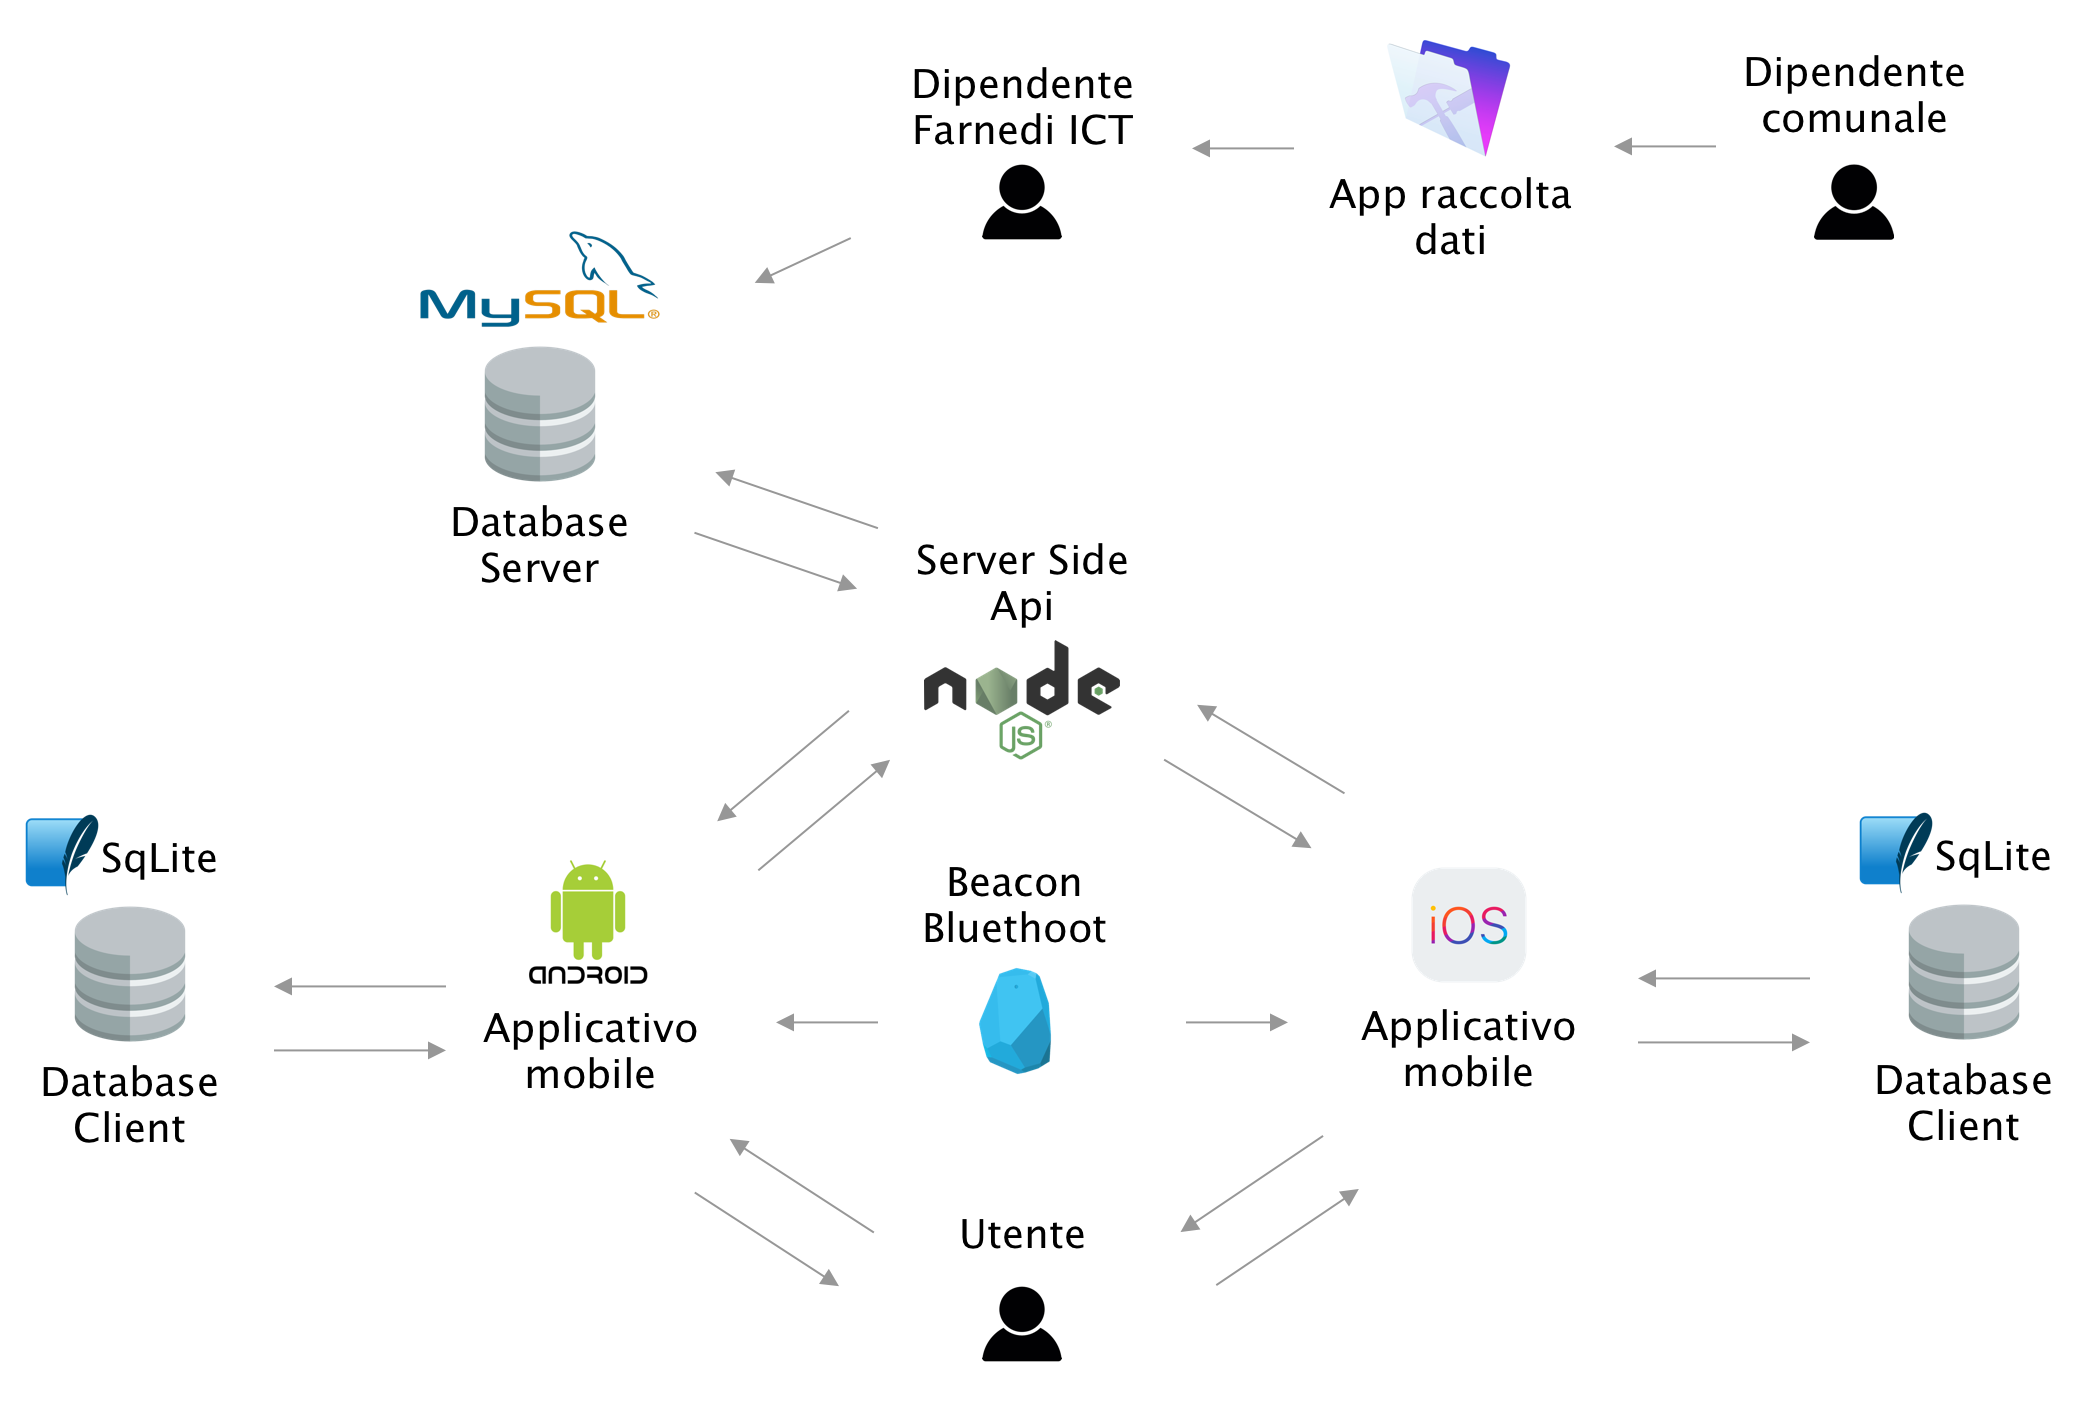
\includegraphics[width=0.8\textwidth]{images/SchemaOpenAirMuseum.png}
\caption{Schema logico dello stack di Open Air Museum}
\end{figure}

\section{Modelli ER}\vspace{5mm}
		
	Il lato server utilizza come database relazionale MySql, che viene sfruttato attraverso un interfaccia Javascript che permette di connettersi al database creando query e inviandole mediante questa connessione. Tutto questo in modo asincrono. Lo schema relazionale per il lato server è presentato in figura 1.2.\vspace{5mm}
	
	Per quanto riguarda le due applicazioni mobile, viene utilizzato sempre un database relazionale, ma sfruttando SqLite come tecnologia, che risulta essere più leggera e adatta a essere eseguita su dispositivi dalle prestazioni ridotte. La figura 1.3 mostra lo schema relazionale per il lato mobile.\vspace{5mm}
	
	[ espandi descrivendo i vari quadrati/entità]\vspace{5mm}

Come si può vedere, la gestione delle funzionalità multilingue dei punti e dei percorsi avviene attraverso una relazione da uno a molti con la tabella 'language'. Questa tabella contiene tutti i testi per lingua supportata. Tale accorgimento è assente nello schema relazionale dei dispositivi mobili dato che, al cambiamento della lingua, le nuove traduzioni verranno scaricate dalle Rest API fornite a lato server.


\begin{figure}[h]
\centering
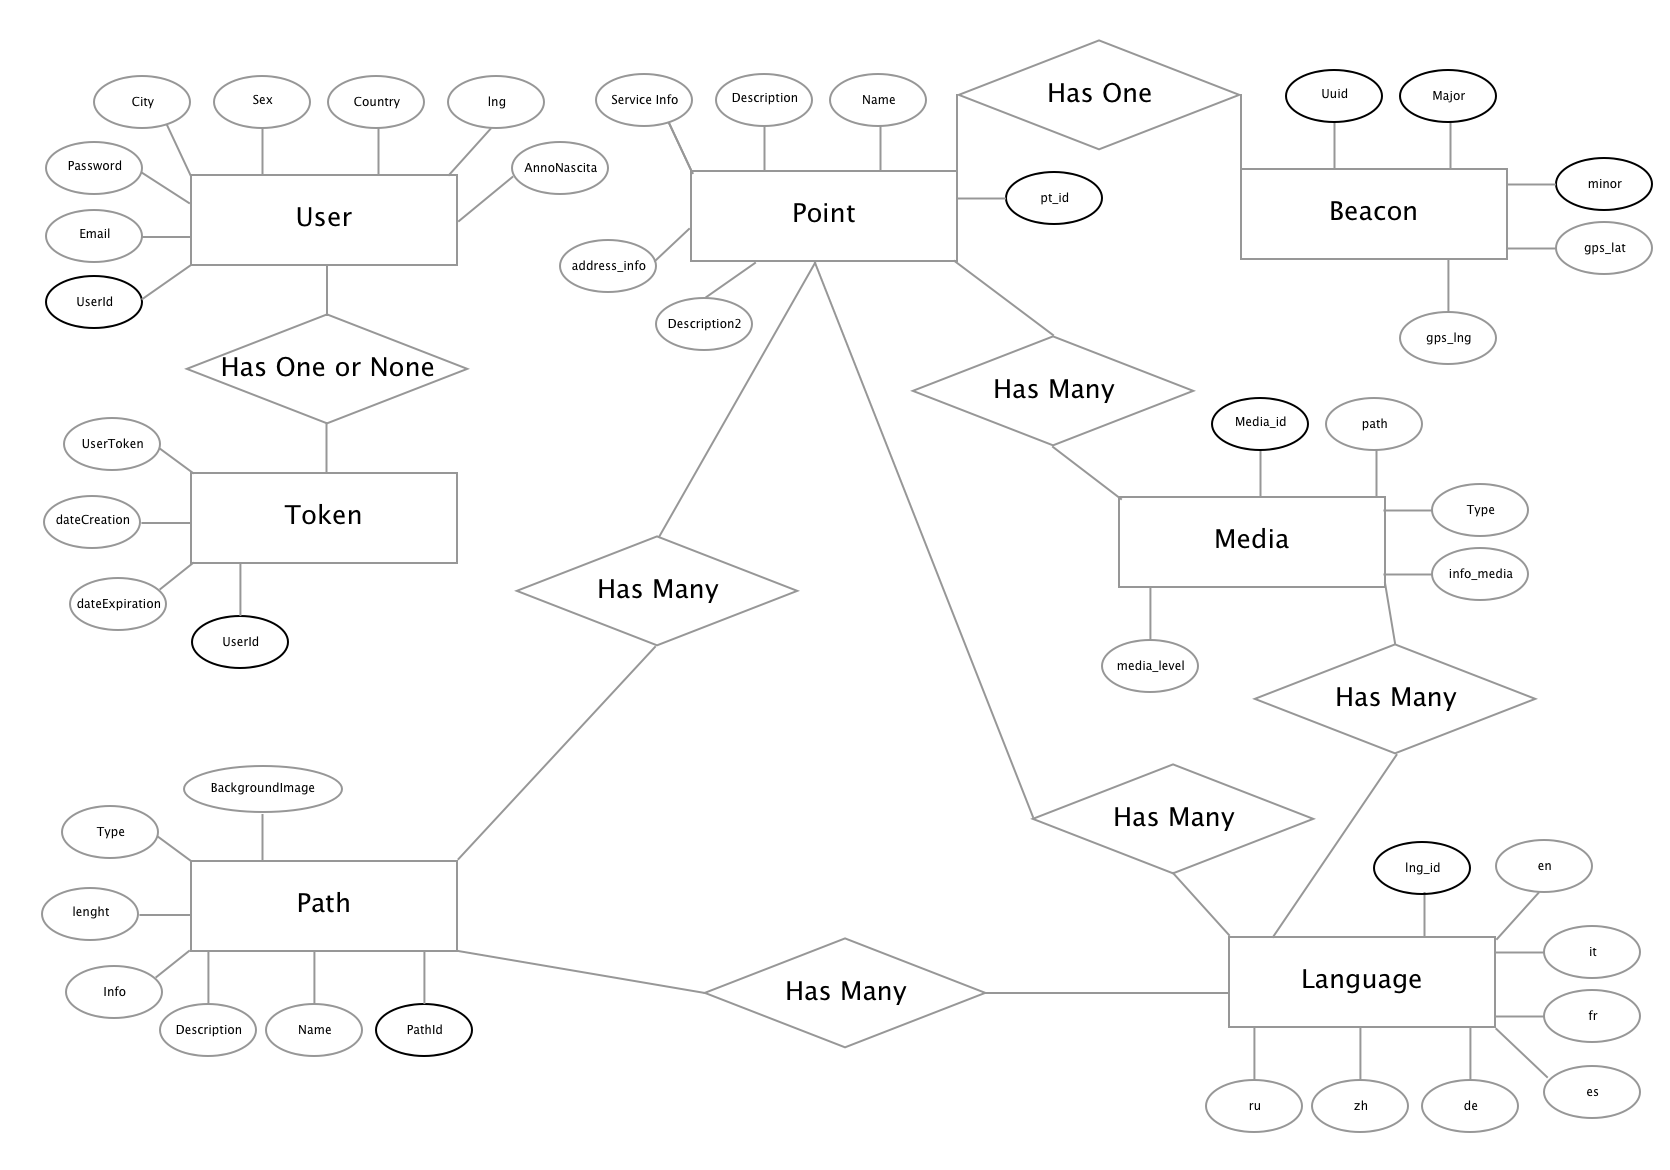
\includegraphics[width=0.8\textwidth]{images/erOld.png}
\caption{Schema ER vecchia versione server}
\end{figure}

\begin{figure}[h]
\centering
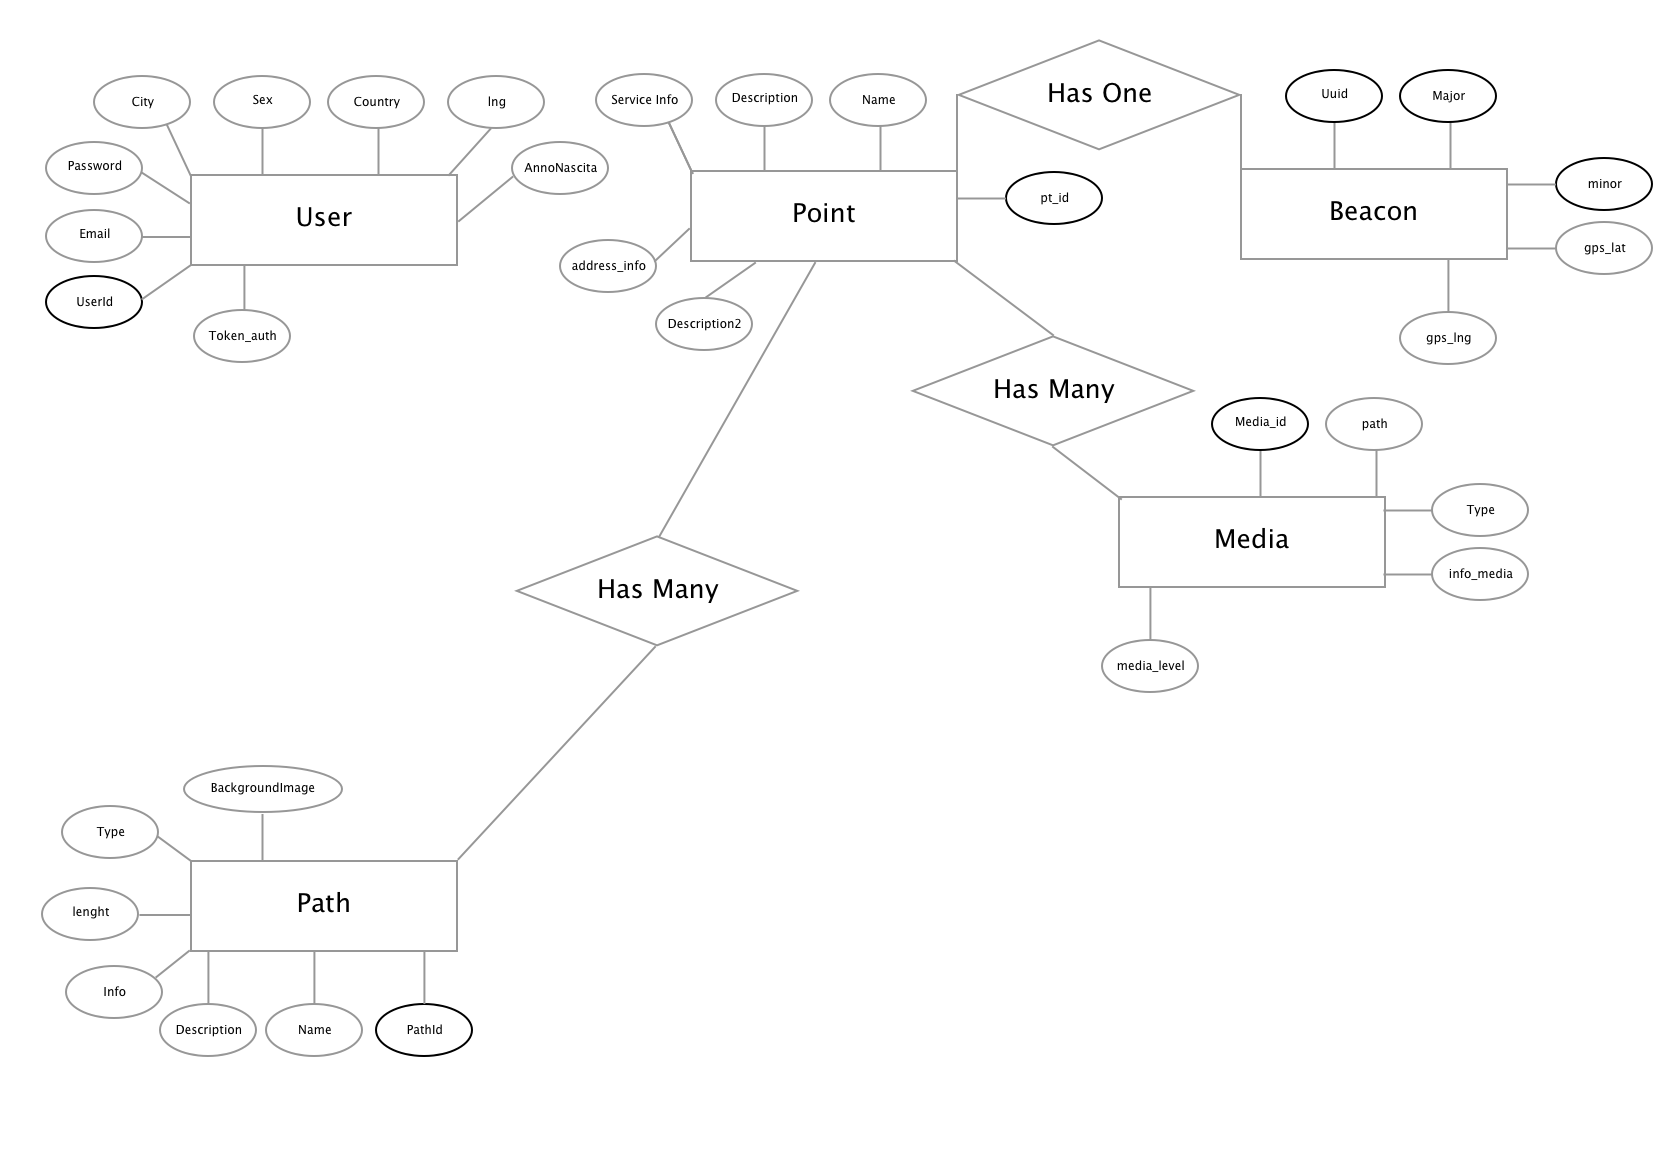
\includegraphics[width=0.8\textwidth]{images/erOldSpartphone.png}
\caption{Schema ER vecchia versione smartphone}
\end{figure}
\vspace{5mm}







      \chapter{Stato dell'arte}
\label{cha:intro}
\vspace{5mm}
\emph{Questo capitolo descrive le varie tecnologie Javascript disponibili sul mercato e in che modo possono essere combinate per costruire il nuovo stack applicativo.}
\section{Javascript}\vspace{5mm}
Javascript è nato come linguaggio di scripting lato client e ha man mano preso piede come uno dei più flessibili e dinamici, diventando uno standard dei browser moderni dichiarando la morte di progetti come Netscape Navigator.\vspace{5mm}

Nel 2009 un ragazzo di nome Ryan Dahl presentò alla JSConf Node Js. Ciò che propose Ryan era quello di utilizzare Javascript come linguaggio lato server utilizzando una strategia simile a quella di Java con la JVM quindi sviluppando un layer di api per utilizzare le risorse del sistema operativo combinato con la flessibilità e la comodità di un linguaggio interpretato.\vspace{5mm}

La vera novità era che per scrivere un applicativo web non bisognava più conoscere due linguaggi (Javascript client e PHP, Java, Python, ecc… server) ma ne bastava uno. Inizialmente la risposta fu tiepida e Node Js rischiò più volte di essere abbandonato, ma con il crescere sempre maggiore della stabilità del framework e la fondazione della Node.js Foundation ad ora è una delle 4 maggiori tecnologie di sviluppo al mondo. L’avvento di questa tecnologia ha incubato una miriade di prodotti diversi dando vita a uno degli ecosistemi più grandi e variegati mai esistiti.\vspace{5mm}

\subsection{Frameworks Javascript}\vspace{5mm}

	L’ecosistema Javascript per il web è molto ricco di soluzioni per tutti gli ambiti di impiego. Per quanto riguarda il lato applicativo front-end vi sono numerose scelte, sia che si intenda operare nel browser che fuori da esso. I principali framework per lo sviluppo web front-end sono React, AngularJs, Vue e Ember. I primi tre implementano il pattern MVC “Model-View-Controller” ovvero la separazione di ciò che detiene i dati da ciò che li renderizza all’utente attraverso una logica che fa da moderatore del flusso. Sia Angular che Vue che Ember offrono nativamente “two-way data binding” ovvero la capacità di mantenere in sincronia tra View e Model. React d’altro canto è stato pensato per essere una libreria e non come un vero e proprio framework infatti il suo approccio è puramente legato alla costruzione dell’interfaccia grafica slegata da quelle che sono tutte le implementazioni possibili nella gestione e nel flusso dei dati. \vspace{5mm}

Nel caso di applicativi complessi che devono gestire molti dati, questa parte può risultare complessa e particolarmente sensibile a bug. Per questo, soluzioni come Redux possono risultare funzionali a tale scope implementativo. Lo scopo di tale libreria è quello di contenere lo stato-applicativo e fare in modo che sia sempre in uno stato certo e consistente permettendo la modifica di esso solo attraverso delle “Action”. Ad ogni “Action” o azione corrisponde una tipologia che il reducer interpreta per modificare lo stato di conseguenza. Il reducer è una funzione pura che prende in input lo stato attuale e l’azione eseguita su di esso e ritorna il nuovo stato applicativo. Essendo i reducer funzioni pure sono prevedibili, prive di “Side effects” e facilmente testabili.\vspace{5mm} 

Per quanto riguarda la parte applicativa per le due piattaforme mobili le scelte possibili sono racchiuse in Cordova/Phonegap, Ionic e React-native. I primi due sono dei “wrap” attorno ad una webView nativa con una serie di Api rese disponibili a Javascript che gira all’interno del browser che risiede nella webView. Tale soluzione è seppur funzionale, non ottimale per il caso d’uso specifico; infatti l’applicativo Alakai necessità di avere accesso al bluetooth e ad altre Api non disponibili negli ambienti di Cordova/PhoneGap. Da notare che Ionic, seppur basato sulla medesima tecnologia mette a disposizione delle Api per interagire in modo completo con il bluetooth, questo e la sua maturità lo rendono un'ottima scelta per sviluppare la parte mobile dell’applicativo.\vspace{5mm} 

D’altro canto React-native è framework basato sull’utilizzo di un motore di compilazione che non fa altro che prendere i costrutti Javascript dichiarati utilizzando librerie e convertirli in codice nativo, a seconda della piattaforma. Inoltre permette, se necessario di interfacciarsi con l’ambiente nativo a piacimento dando la possibilità di utilizzare un costrutto chiamato “bridge” che offre un’interfaccia a Javascript verso il nativo e viceversa. La differenza principale tra i sistemi che usano Cordova e React-native è che il primo ha come goal quello di “Write once run everywhere” mentre il secondo è “Learn once use everywhere”.\vspace{5mm}

Per la parte server vi sono disponibili anche qui diverse scelte e tecnologie, seppur orientate alla stessa soluzione molto diverse tra di loro. Vi sono librerie come Express js che sono pensate per essere molto leggere e di lieve impatto nella strutturazione dei dati. Di contro ve ne sono altre che offrono un profondo controllo su tutti gli aspetti dell’applicativo come MeteorJs e Sails Js che offrono una serie di features come la generazione automatica di Api seguendo la specifica delle “CROUD operation”, la generazione automatica di modelli per descrivere nuove entità e la gestione automatica dell’autenticazione e la gestione degli utenti.\vspace{5mm}

\section{Sviluppo mobile}\vspace{5mm}

Al giorno d'oggi sono disponibili sul mercato una vasta gamma di smartphone che variano per dimensione e potenza. Tali applicativi permettono di utilizzare software proveniente da terze parti, installabili mediante uno store digitale messo a disposizione, solitamente, dal mantenitore del sistema operativo. Tali software sono indicati con il nome di Apps o Application.\vspace{5mm}

I metodi canonici per lo sviluppo di Apps con queste tecnologie sono l'utilizzo dei tool messi a disposizione dal mantenitore del sistema operativo e cioè, XCode e Android studio. Ogni sistema operativo ha a disposizione un sdk che permette di sfruttare l'hardware del dispositivo; tale sdk però è relegato ad un solo sistema operativo, con molte differenze, sia tecniche che logiche, tra i due. Un ulteriore differenza è il linguaggio, iOS utilizza ObjectiveC o Swift mentre Android Java o Kotlin. Tali dissomiglianze portano a dover, nel caso si desideri sviluppare per entrambi i sistemi operativi, a conoscere entrambi i linguaggi e i rispettivi sdk.\vspace{5mm}

\subsection{Sviluppo mobile e Javascript}\vspace{5mm}

Ciò che Javasctipt e il web in generale ha portato allo sviluppo nativo è l'approccio del 'write one run anywhere' e cioè la possibilità di avere una codebase unica per più sistemi operativi. Javasctipt negli anni si è posto come 'lingua franca' del Web e in grado di raggiungere zone molto lontane da quella per cui era stato originariamente progettato. Il parco di framework che offrono questo tipo di approccio sono molteplici e implementano tecniche differenti per raggiungere il medesimo scopo:
\begin{itemize}
\item Soluzione Ibrida
\item Soluzione Compilata
\end{itemize}

La prima utilizza un approccio ibrido e cioè l'applicativo è di fatto una applicativo web che viene eseguito all'interno di un browser che ha però capacità speciali di interazione con l'hardware dello smartphone. Di fatto offre un layer al di sopra degli sdk nativi che permettono alla web app di accedere a funzionalità native come il bluethoot e la fotocamera.\vspace{5mm}

La soluzione compilata invece utilizza uno stratagemma diverso. Tutti i componenti descritti in Javascript attraverso una particolare interfaccia vengono compilati dal framework che gli converte in componenti nativi, mentre la logica applicativa viene lanciata su di un thread separato che comunica attraverso un costrutto software con la controparte nativa. Tale approccio permette di avere prestazioni più elevate e maggior flessibilità rispetto all'ibrido ma risulta più complesso, non essendo presenti layer che astraggono i rispettivi sdk ma è necessario seguire le direttive imposte dal sistema operativo.


\section{Audioguide}\vspace{5mm}

Vi sono disponibili diversi prodotti che offrono la possibilità di creare audioguide per determinate zone o città. Alcuni di questi utilizzano un approccio di “selezione luogo” e cioè chi utilizza l’applicativo deve prima indicare a quale zona è interessato per poi essere reindirizzato alla sezione relativa a quell’area geografica. Altri prodotti come Open Air Museum utilizzano un approccio “mono scopo” e cioè l’audioguida è relativa ad una sola area specifica e sviluppata ad Hoc per quello scopo. L’approccio descritto per primo permette di dover mantenere un solo prodotto e di servire molteplici enti, questo però limita molto la customizzazione che tali applicativi possono possedere. Di contro il secondo approccio permette una customizzazione elevata, essendo il prodotto sviluppato appositamente per l’ente; questo però comporta un overhead non indifferente per chi mantiene tale applicativo. Infatti se si vogliono servire un gran numero di realtà risulta dispendioso dover gestire e mantenere molti applicativi diversi, ognuno con le sue peculiarità e caratteristiche.\vspace{5mm}

Un ulteriore punto di riflessione sono le funzionalità. La totalità dei competitor presi in considerazione permette di visualizzare contenuti multimediali collegati a punti di interesse o percorsi, ma in pochi offrono un servizio di localizzazione attivo a guidare all’interno della zona di interesse. La totalità degli applicativi presi in considerazione che hanno questa features utilizzano come tecnologia di localizzazione il gps che per zone all’aperto, come lo possono essere città o parchi naturali, è un ottima soluzione; però per quanto riguarda la localizzazione indoor come in un museo per esempio, risulta imprecisa e poco utilizzabile. IBeacon in questo caso risulta la tecnologia migliore per localizzazione degli utenti dato che non deve fare affidamento a triangolazioni satellitari.\vspace{5mm}

Quello che offrirà al nuova versione di Open Air Museum è un approccio misto rispetto a quello descritto all’inizio di questo capitolo, ciò che si andrà a realizzare andrà a rientrare nella categoria “mono scopo” ma grazie all’elevata flessibilità delle impostazioni di avvio sarà possibile customizzare in modo profondo l’applicativo mantenendo allo stesso tempo una documentazione esplicita sulle proprie features. Infatti il file di configurazione è in formato Json\cite{JSON} quindi facilmente accessibile sia ad umani sia a computer.\vspace{5mm}





      \chapter{Strumenti e tecnologie}
\label{cha:intro}
\vspace{5mm}

\emph{Questo capitolo descrive in maniera più approfondita le tecnologie utilizzate nella prima e nella seconda versione in un confronto dettagliato.}

\section{Tecnologie utilizzate in Open Air Museum}\vspace{5mm}

Indicherò le varie tecnologie utilizzate per l'attuale versione dell'applicativo.\vspace{5mm}

\subsection{Filemaker}\vspace{5mm}

Filemaker è una piattaforma per creare applicativi personalizzati votati alla categoria “gestionale” sviluppata da Apple. Open Air Museum utilizza questa tecnologia per creare l’interfaccia per la raccolta dati che verrà utilizzata da alcuni addetti comunali che appunto arricchiranno l’applicativo con i testi e i media provenienti da questo software. Tale applicativo è standalone e quindi slegato dall’applicativo lato server che espone le Api e l’importazione dei dati provenienti da questa soluzione deve essere fatta manualmente. Ciò comporta uno svantaggio non indifferente che preclude una scalabilità rapida del prodotto. La scelta di questa tecnologia era quella di avere il più rapidamente possibile un prodotto in grado di iniziare a raccogliere dati il prima possibile e qualunque altra soluzione, seppur migliore in un ottica futura, avrebbe impiegato maggior tempo di sviluppo.\vspace{5mm}

\subsection{Node Js}\vspace{5mm}

	Come descritto in precedenza, Node js è un runtime di Javascript al di fuori del browser.Tale programma, come dicuterò più avanti, utilizza Chrome V8\cite{V8} come motore per eseguire Javascript ed grazie ciò NodeJs è stato fornito di una suite di interfacce per la comunicazione con l'hardware. In particolare questa particolare implementazione viene indicata come I/O non bloccante\cite{AsincIO}. La particolarità di questa soluzione è che mette a disposizione una serie di Api a basso livello che permettono di utilizzare la scheda di rete e quindi di avviare server TCP e HTTP oltre che accesso al file system quindi lettura e scrittura su disco. In Open air museum questo framework è utilizzato per costruire il lato server ed esporre una serie di Api Http Rest che permettono la fruizione dei dati. Tutti i media, quindi audio e immagini vengono serviti anch’essi da questa piattaforma che oltre a questo gestisce anche l’autenticazione degli utenti e la gestione degli stessi. \vspace{5mm}
	
	\subsection{Estimote}\vspace{5mm}
	
	\subsection{Developer Tools}\vspace{5mm}
	
	[RISCRIVI QUESTA PARTE.]

	Xcode è una Ide per lo sviluppo IOS. L’applicativo per tale sistema operativo è stato sviluppato in Swift4.\vspace{5mm}

	Android Studio è una Ide per lo sviluppo Android. L’applicativo per tale sistema operativo è stato sviluppato in Java per android.\vspace{5mm}

	MySql/SqLite sono le tecnologie che utilizzano i due database relazionali di cui il prodotto è fornito. Tutti i dati lato server sono contenuti in un database MySql che viene pilotato tramite l’applicativo lato server in Nodejs. Entrambi i database lato client utilizzano invece SqLite. 
	
	Visual Studio Code
	
	Github
	
	Bitbucket?
	
		\subsection{Modello ER}\vspace{5mm}
		
	Lo schema relazionale per il lato server è il seguente, si vedano gli allegati per i due(???) schemi ER corrispondenti. [ESPANDI?]  \vspace{5mm}
	
\begin{figure}[h]
\centering
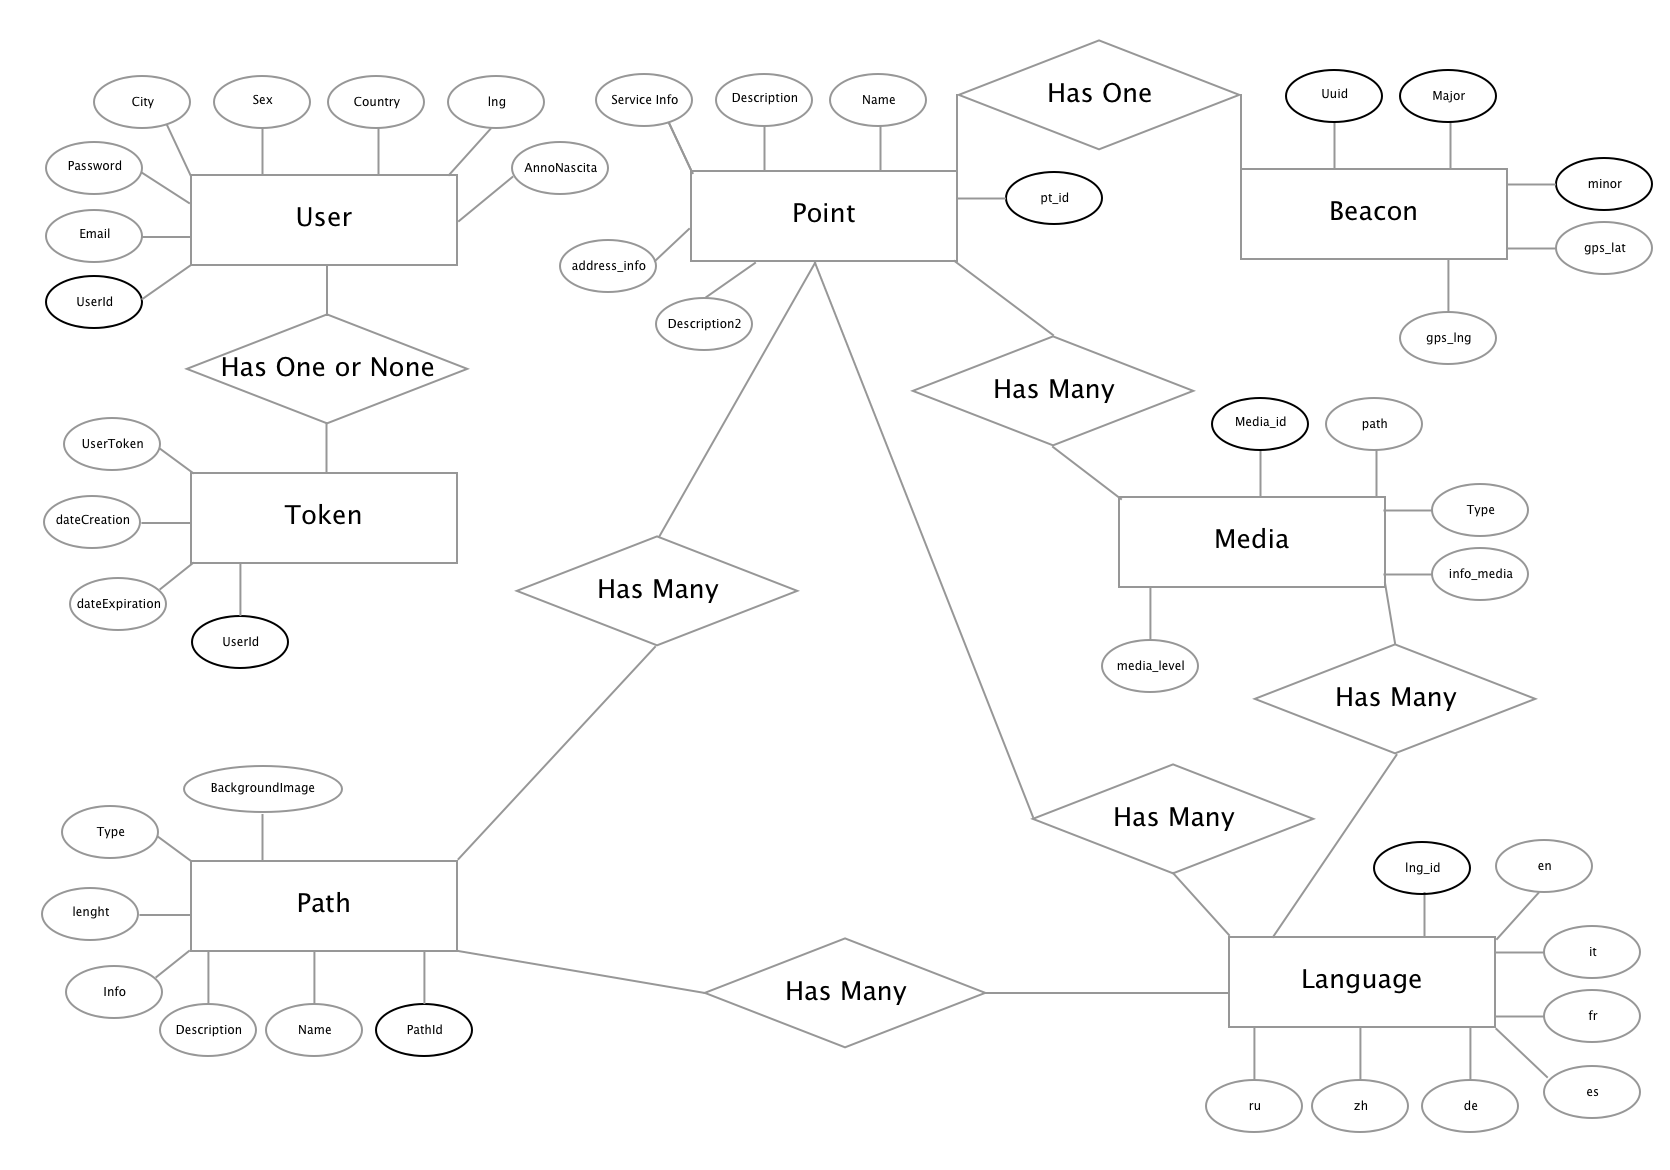
\includegraphics[width=0.9\textwidth]{images/erOld.png}
\caption{Schema ER vecchia versione}
\end{figure}
\vspace{5mm}

[mi sa che manca uno schema.]
	
\section{Tecnologie versione 2.0}\vspace{5mm}
Indicherò le varie tecnologie utilizzate per la nuova versione dell'applicativo ponendo particolare attenzione a che vantaggi portano.\vspace{5mm}

	\subsection{React}\vspace{5mm}

React è una Libreria Javascript per lo sviluppo di interfacce grafiche a componenti, permette lo sviluppo di single page application (SPA). In Alakai l’applicativo che permette l’inserimento dei dati e dei media oltre alle descrizioni dei punti di interesse e dei percorsi è creata utilizzando questa tecnologia sfruttando un set di Api che il lato server fornisce. Questo centralizza la gestione dei dati in un unico luogo e cioè il server, tale approccio permette di utilizzare l'applicativo backend come unica fonte di verità senza dover gestire due prodotti separati come vi era in precedenza. [ESPANDI!!!]\vspace{5mm}

	\subsection{Redux}\vspace{5mm}
	
	Redux è una libreria Javascript che permette di gestire lo stato applicativo come un unico oggetto statico, modificabile soltanto attraverso della azioni ben definite applicate ad esso. Ogni modifica viene fatta attraverso una funzione pura\cite{PureFunction} chiamata reducer che modifica a seconda dell'implementazione una parte specifica dello store. La firma di tale funzione prende due parametri, il primo è l'oggetto che rappresenta lo stato attuale dell'applicativo, il secondo è ciò che rappresenta l'azione che si sta compiendo. Tale azione dovrà sempre possedere una tipologia mentre può o non può avere un payload di dati che si riferiscono a quell'azione specifica. Ciò che ritornerà il reducer sarà un oggetto che diventerà il nuovo stato applicativo. Questa tecnologia è utilizzata per gestire i dati che gli applicativi mobile recupereranno dal server in modo predittivo e sicuro. Tale implementazione permette di evitare side effects\cite{SideEffects} nello stato applicativo facendo si che l'unica fonte di verità sia sempre affidabile e prevedibile.  [ESPANDI!!!] \vspace{5mm}
	
\begin{figure}[h]
\centering
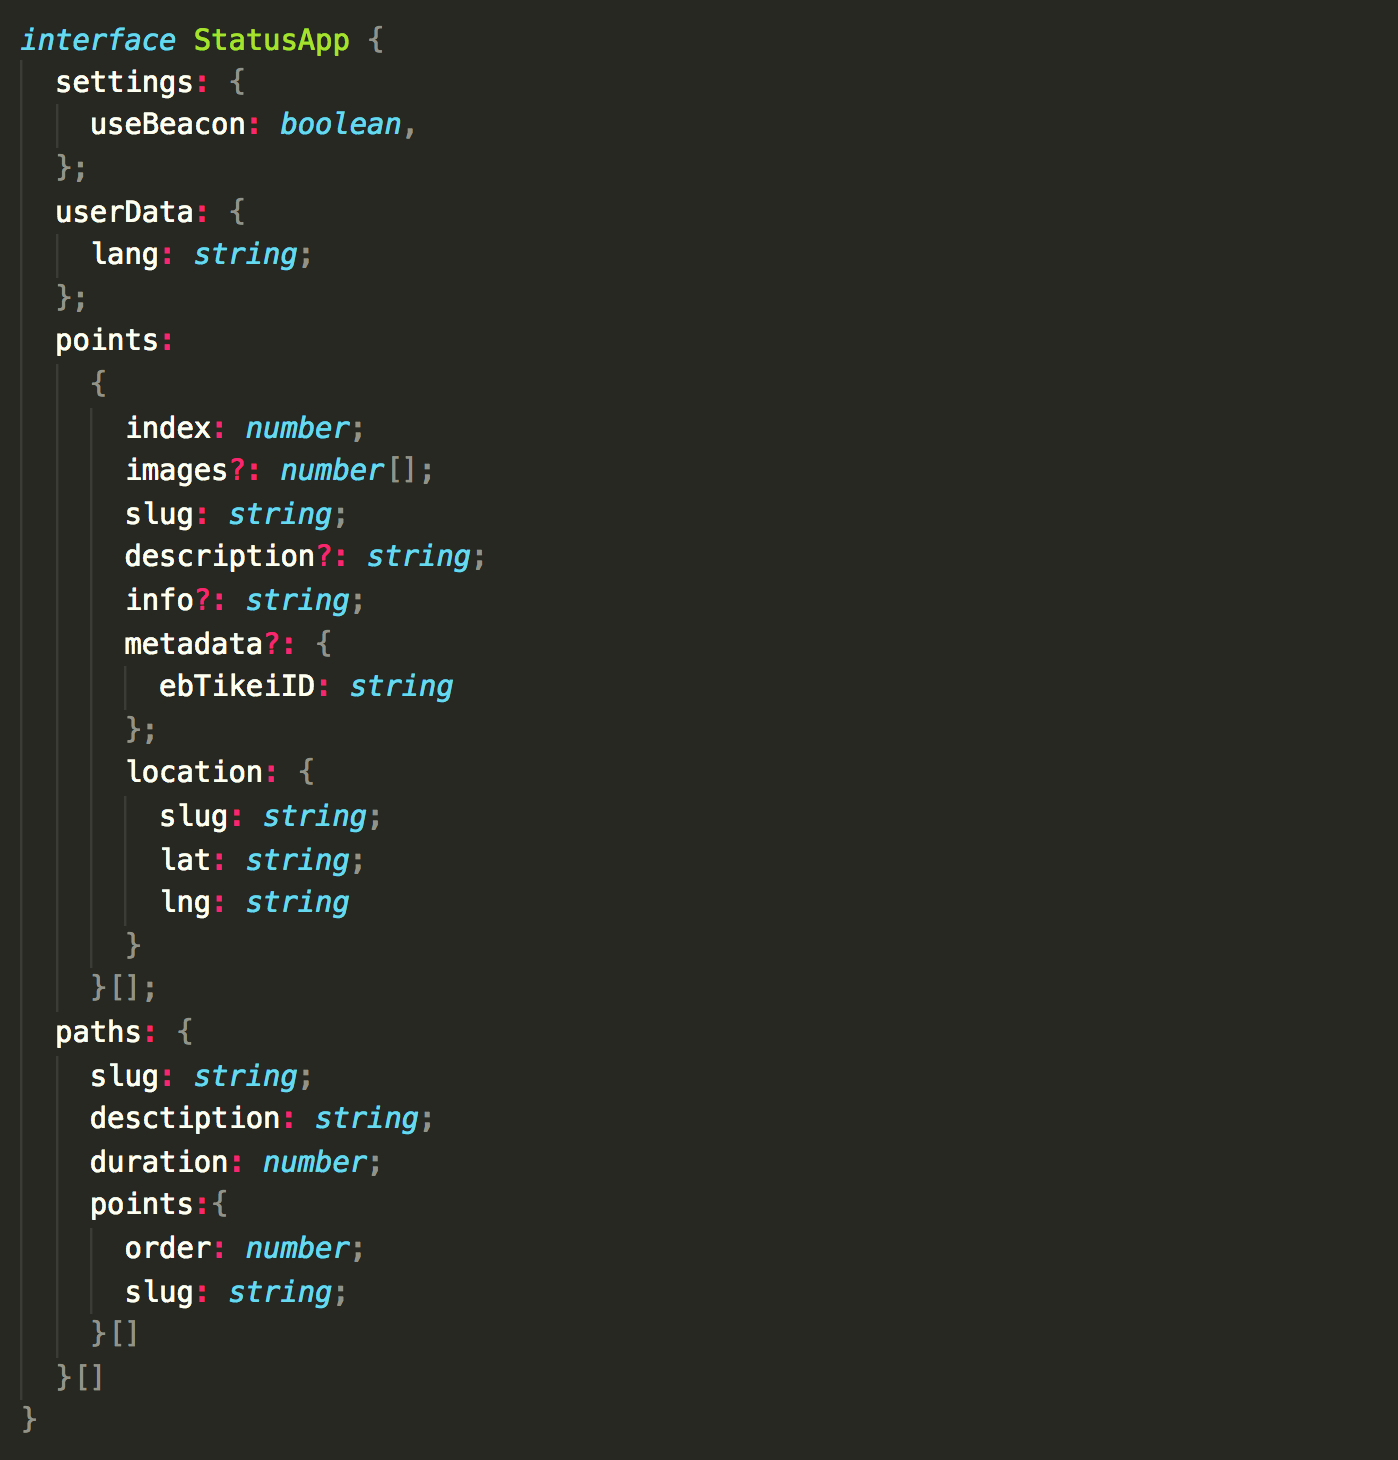
\includegraphics[width=0.7\textwidth]{images/store.png}
\caption{Interfaccia Store Redux}
\end{figure}
\vspace{5mm}

\subsection{React-Native}\vspace{5mm}

	React-Native è l'implementazione di React ma per l’ambiente nativo. Questa tecnologia verrà usata per creare l’interfaccia e la logica degli applicativi IOS e Android. Tale scelta infatti permette di condividere buona parte del codice tra le due piattaforme.\vspace{5mm}

\subsection{Express}\vspace{5mm}

	Express è l'implementazione del pattern middleware per Node Js. Tale framework permette di gestire con granularità il routing delle Api e da la possibilità di centralizzare la gestione degli errori. L'implementazione di tale pattern si riflette in un applicativo che esegue le computazioni attraverso una cascata di funzioni chiamate una dopo l'altra in ordine, ed ognuna di esse ha la facoltà di decidere se continuare la catena o interrompere la computazione. Questo permette di avere una struttura affidabile per gestire il routeing delle Rest api rendendo molto veloce e predittivo lo sviluppo.\vspace{5mm}

\subsection{SqLite}\vspace{5mm}

	SqLite è “File-based” database utilizzato lato server per il salvataggio delle informazioni fornite dagli utenti admin attraverso l’applicativo web per la raccolta dei dati. Tale scelta è stata fatta per la flessibilità di questa tecnologia che permette di gestire internamente all’applicativo la creazione dello stesso e non attraverso una dipendenza esterna. Questo è stato fatto per semplificare ulteriormente il deploy eliminando le necessità di aggiungere una configurazione ulteriore all’ambiente.\vspace{5mm}
	
	\subsection{Modello ER}\vspace{5mm}

Ora descriverò brevemente il nuovo schema logico dell'applicativo e come le varie tecnologie, tutte basate su Javascript interagiscono fra loro.
	
\begin{figure}[h]
\centering
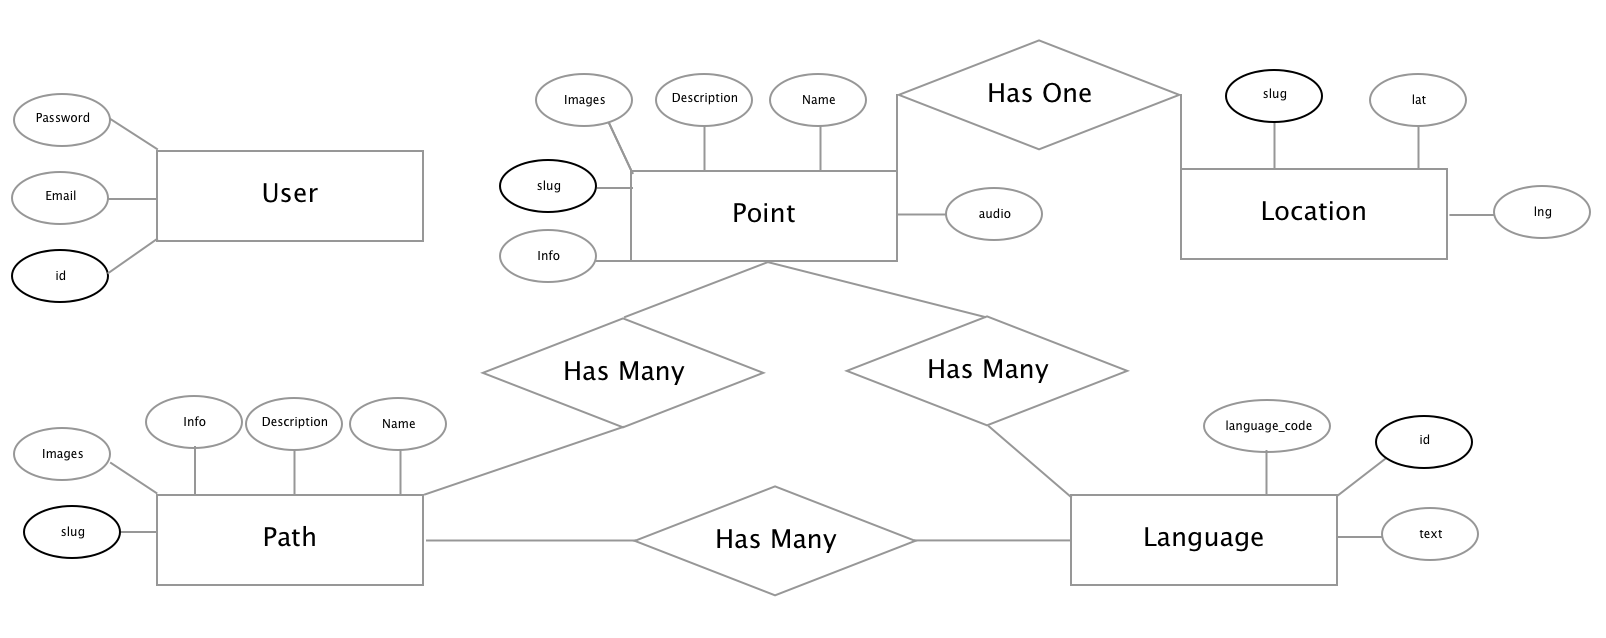
\includegraphics[width=0.9\textwidth]{images/erNew.png}
\caption{Schema ER nuova versione}
\end{figure}
	
	
\begin{figure}[h]
\centering
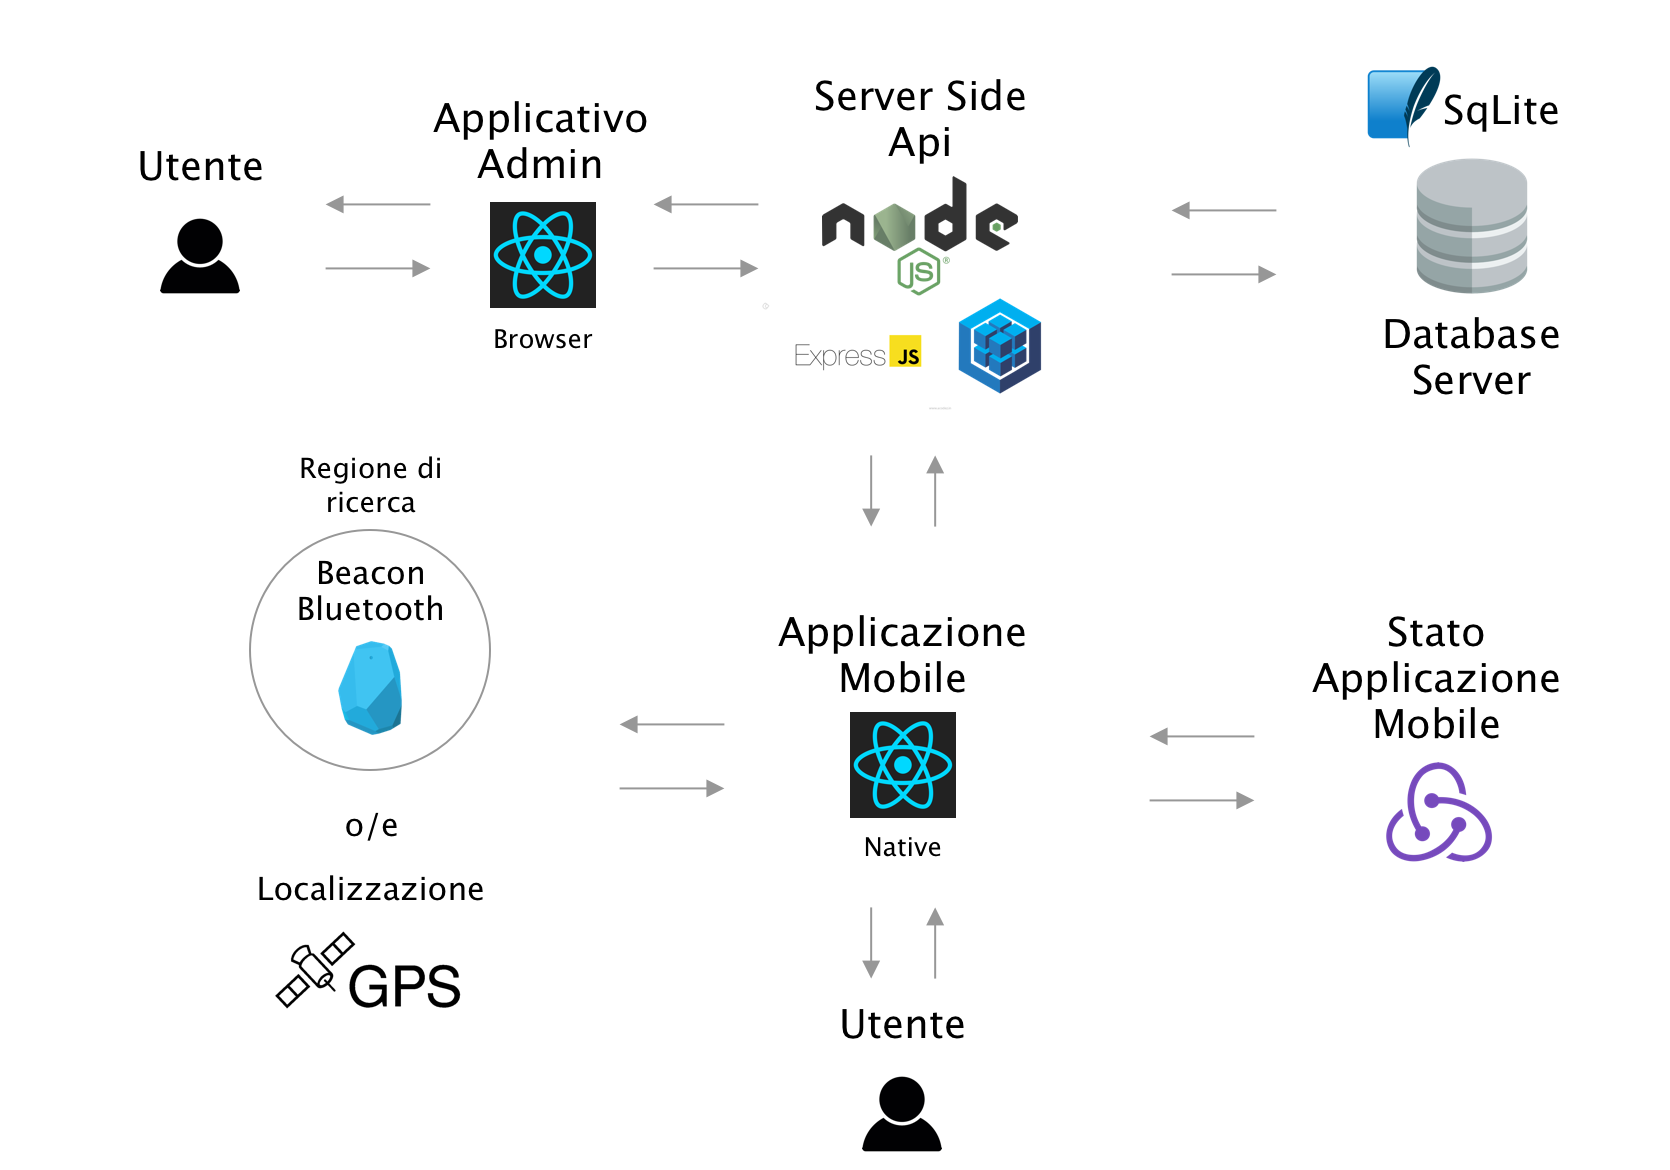
\includegraphics[width=0.9\textwidth]{images/stackAlakai.png}
\caption{Schema stack nuova versione}
\end{figure}

\vspace{5mm}Come si può vedere in figura 2.4 lo stack risulta meno complesso e vanta l'utilizzo di meno tecnologie per raggiungere le medesime funzionalità. Come si può notare i punti di interazione con la piattaforma sono gestiti da due applicativi basati entrambi su React, il primo è l'applicativo mobile che utilizza React-native mentre il secondo è la webApp admin. Entrambi questi applicativi ricevono input dall'utente ma il primo utilizza hardware esterno per arricchire la propria raccolta informazioni con la posizione dell'utente, ricevuta attraverso il gps o Beacon bluethoot. Tali applicativi interagiscono con il server mediante delle Rest Api che, come nella versione precedente, forniscono i dati sui punti e i percorsi; ma, in contrasto con l'applicativo prima del refactor, portano anche la configurazione impostata dall'applicativo admin in modo da adattarlo alle richieste di chi gestisce i punti e i percorsi. Tali dati vengono salvati in un database SqLite il cui unico punto di accesso è attraverso le api fornite dal server. \vspace{5mm}

Tale approccio garantisce che i dati siano sempre consistenti con quello che è l'applicativo server in modo da mantenere la struttura consistente con il versionamento del prodotto. Un ulteriore struttura per mantenere i dati è presente a lato mobile mediante Redux, questo è utile per poter salvare le configurazioni e mantenerle tali in modo consistente attraverso l'app in modo da creare una coesione tra tutti i componenti di React che necessitano di usufruire dei dati. Tale stato applicativo viene idratato attraverso le api Rest e quando questo non è possibile per mancanza di rete permette di utilizzare tramite React-native lo Storage locale del dispositivo come luogo di backup. Ogni mutazione dello stato applicativo viene infatti seguita da un operazione asincrona che ha lo scopo di salvare uno snapshot dello store nella memoria del dispositivo in modo da poter essere sempre consistente nel mostrare gli ultimi dati disponibili anche se il dispositivo risulta offline.\vspace{5mm}

\section{Confronto tra le due versioni}\vspace{5mm}  
[forse questo va piu nelle conclusioni?]

Confrontando gli stack delle due applicazioni in termini di tecnologie utilizzate possiamo vedere i motivi per cui le scelte fatte migliorano il software e sotto quali aspetti. \vspace{5mm}

Grazie all'utilizzo del medesimo framework lato mobile e lato web è stato possibile condividere gran parte del codice e delle logiche di interazione con le api lato server. Un altra zona di condivisione è l'implementazione di Redux. Data la sua agnosticità sulla piattaforma utilizzata questa libreria è un perfetto esempio di come l'utilizzo di uno stack basato interamente su Javascript porti ad un riutilizzo del codice in modo importante ma sopratutto in modi impraticabili precedentemente. In particolare tra l’applicativo admin sviluppato come webapp per il browser e gli applicativi nativi ho condiviso la totalità dell’implementazione gestendo lo store allo stesso modo. Le differenze principali sono sulla libreria che permette di interfacciarsi con le api lato server. Seppur molti metodi sono condivisi, quelli relativi alla mutazione dei dati sono riserveti ai soli utenti autenticati e cioè Admin. Tale peculiarità però non influisce nella possibilità di riutilizzare parte della libreria che implementa sia i metodi lato amministratore che quelli lato utente senza privilegi.\vspace{5mm} 

Un ulteriore punto è che rispetto alla versione precedente vi è una somiglianza molto forte tra quello che è l’applicativo web e l’applicativo nativo, le due applicazioni non sono compatibili ma condividono gran parte delle logiche e dei pattern essendo di fatto lo stesso framework. Ciò permette di avere un livello di complessità all'approccio a questo progetto più bassa della versione precedente. Questo porta a tempi più corti per l'apprendimento dei pattern e delle logiche e di conseguenza risulta in una miglior produttività.\vspace{5mm}
	
La scelta dell’utilizzo di un database a file con la possibilità di configurare e passare ad un database “classico” si è rivelata molto importante per la scalabilità dell’applicativo. SqLite risulta più comodo in fase di deploy di contro, non ha le prestazioni di un database “classico” e la possibilità di configurare rapidamente la tecnologia da utilizzare è un plus importante. Questo si ottiene grazie all’impiego di un ORM in grado di fornire questa features come Sequelize. Oltre a questo permette di implementare in modo veloce migrazioni e seeder restando sempre agnostico sulla tecnologia a database. La versione precedente conteneva una pesante assunzione sull’utilizzo di un database MySql e ciò abbassava sostanzialmente la flessibilità e il riutilizzo del prodotto.\vspace{5mm}

Un altra differenza rispetto alla precedente è l’esistenza dell’applicativo admin in react che dovrà essere servito dall’applicativo server. Per fare questo è necessario che tutte le richieste non inviate direttamente a /api, vengano tutte reindirizzare all’applicativo in modo che la SPA utilizzi il router interno a React per mostrare i contenuti corrispondenti all’url della richiesta.\vspace{5mm}

Riguardo al lato “admin”, cioè quello che va a sostituire Filemaker nella raccolta dati, è stato sviluppato con React. La scelta di sviluppare una SPA\cite{SPA} per questo compito è stata dettata da un bisogno di rendere questa operazione iterabile e ripetibile. Nel caso in cui il cliente volesse cambiare dei testi o correggere delle traduzioni può farlo in autonomia, senza dover passare da una figura che traduca le modifiche richieste aggiungendole a database manualmente. Questo processo inoltre astrae ulteriormente la struttura del database durante il processo di inserimento dei dati offrendo quindi flessibilità su modifiche future alla struttura. Un altro punto a favore della scelta di una SPA \vspace{5mm}


      \chapter{Porting a React-native}
\label{cha:intro}
\vspace{5mm}

\emph{Qui descriverò nel dettaglio il porting degli applicativi nativi a React-native, descrivendo il percorso implementativo e riassumendo i punti critici.}
\vspace{5mm}
\section{Caratteristiche principali}\vspace{5mm}

La caratterizzazione fondamentale di questo tipo di porting è quello di non compromettere la funzionalità iniziale dell’applicativo, mantenendo un “lookAndfeel” il più possibile vicino all’applicativo iniziale, ma apportando allo stesso le possibili migliorie date dal nuovo ambiente. La prima problematica affrontata è stata quella di poter gestire la modalità Esplora da Javascript e cioè essere in grado di controllare il bluetooth dello smartphone e mediante una task in background monitorare l’avvicinarsi o meno a specifiche aree marcate da un dongle. La tecnologia di comunicazione bluetooth supportata dalla versione nativa era IBeacon mediante un SDK sviluppato da Estimote. La decisione di mantenerla anche nel porting è stata data dall hardware gia configurato e presente sul territorio. Come detto in precedenza la comunicazione tra il reame nativo e quello Javascript avviene attraverso una particolare struttura software chiamata bridge. Tramite le Api messe a disposizione da react-native è possibile utilizzare questa struttura per passare dati tra i due reami. Ora descriverò nel dettaglio in che modo utilizzare tali api per garantire nel reame Javascript le stesse Api dell’SDK Estimote proximity, sia su iOS che su Android.\vspace{5mm}

Per quanto riguarda iOS è necessario aggiungere alle dipendenze del progetto Estimote Proximity SDK, mediante CocoaPods, un dependency manager per XCode. Inoltre è necessario per abilitare la localizzazione in background aggiungere tra le “Capabilities” dell’applicativo nella la voce “Background Mode” la voce “Uses Bluetooth LE accessories”. \vspace{5mm}

A questo punto è necessario creare un file che permetta di dichiarare ed esportare i metodi di configurazione e gestione della libreria dichiarandoli utilizzando l’interfaccia fornita da RCTBridgeModule  di react-native per renderli visibili lato Javascript al momento della compilazione e dell’esecuzione dell’applicativo. Un ulteriore punto importante è che la comunicazione attraverso il “bridge” è asincrona e per questo è possibile passare valori da nativo a javascript mediante callback o eventi. \vspace{5mm}

Nel caso specifico la scelta è ricaduta su di un sistema ad eventi, per la maggior flessibilità di utilizzo. In particolare i metodi messi a disposizione attraverso il “bridge” sono:
\begin{itemize}
	\item initialize:(NSDictionary *)config
	\item startObservingZones:(NSArray *)zonesJSON
	\item stopObservingZones()
\end{itemize}
	\vspace{5mm}
Il primo ha lo scopo di inizializzare l’sdk Estimote attraverso un oggetto che contiene i vari parametri di configurazione. Il secondo permette di mettere il device in ascolto su una lista di zone identificate mediante dei tag, quando il telefono entrerà in una zona così configurata verrà lanciato l’evento “Enter”. Per l’uscita da una regione verrà lanciato l’evento “Exit” mentre per un cambio di contesto mentre si è in una zona verrà lanciato “Change”. Il contesto è un parametro passato nella funzione chiamata dalla sottoscrizione a questi eventi e contiene le informazioni del beacon che rappresenta quella regione.\vspace{5mm}

Per quanto riguarda Android lato Javascript le api sono le medesime per dare una sensazione di uniformità tra le due piattaforme. Per quanto riguarda l’implementazione nativa l’implementazione dell’sdk avviene in modo paritetico che con ios ed anche l’esportazione dei metodi attraverso il “bridge”; ciò che cambia effettivamente sono le configurazioni necessarie date da un ambiente diverso (Java).\vspace{5mm}

A questo punto mediante un interfaccia messa a disposizione da React-native e possibile quindi utilizzare i metodi esportati dalle due piattaforme. Tali metodi sono esportati attraverso l’oggetto ”NativeModules” che a sua volta contiene un oggetto per ogni classe che implementa l’interfaccia RCTBridgeModule. A questo punto è stato scelto utilizzare un file Javascript che normalizza l’esportazione dei vari metodi e nel caso in cui vi siano differenze tra una piattaforma e l’altra è bene esportare solamente quelli disponibili per quel Sistema operativo. Nel caso di questa particolare implementazione le api sono paritetiche per cui non sono stati necessari accorgimenti specifici.\vspace{5mm}

Voglio far notare che, seppur i due sistemi operativi sono molto differenti, le api lato Javascript risultano paritetiche. Questo offre un astrazione che elimina la complessità di dover gestire singolarmente due linguaggi diversi con ambienti diversi. React-native offre mediante le “Bridge Api” la possibilità di costruire librerie non “cross platform” ma “multi platform”. Tale valore non è indifferente e può risultare cruciale per quanto riguarda tempi di sviluppo e features del prodotto dando la possibilità di scrivere solo il codice nativo necessario, sviluppando poi il resto della logica in un'ottica “write once run anywhere”.\vspace{5mm}

Dal punto di vista grafico inoltre sono state apportate molte modifiche dati i feedback di molti utenti che trovavano l’applicativo precedente poco intuitivo. Si è passati da una visualizzazione dei punti di interesse da lista a mappa. Infatti molti utenti si lamentavano del fatto che non era immediato capire dove fossero i punti rispetto alla loro posizione.\vspace{5mm}

\begin{figure}[h]
\centering
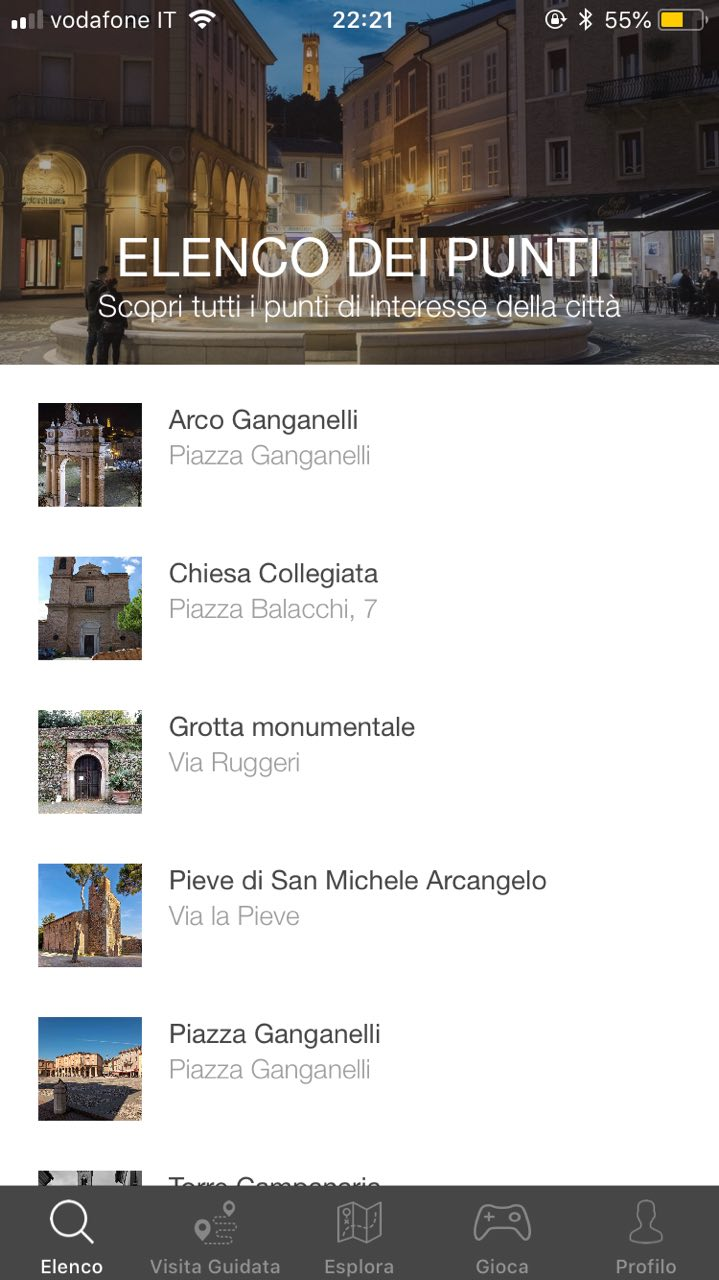
\includegraphics[width=0.3\textwidth]{images/screenSantarcangelo.jpg}
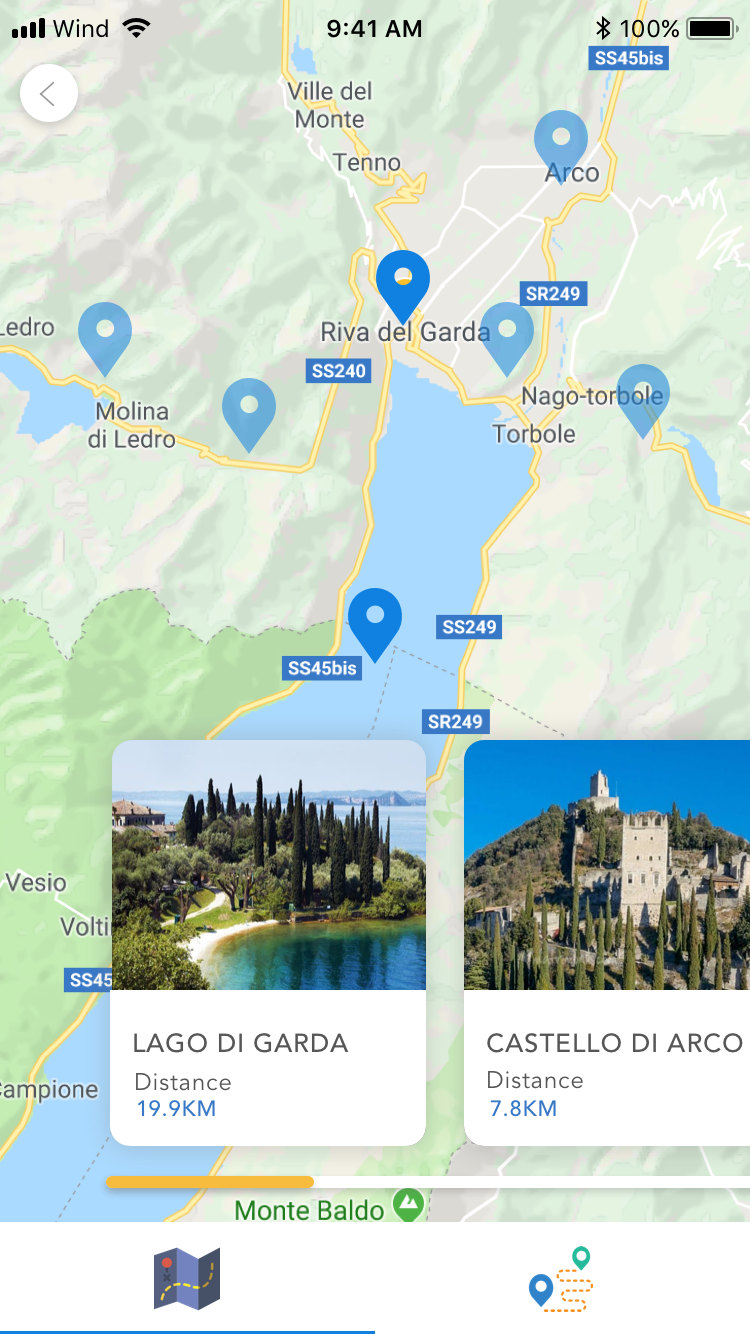
\includegraphics[width=0.3\textwidth]{images/listapunti.png}
\caption{Confronto HomeScreen Open Air Museum vecchia e nuova versione}
\end{figure}
\vspace{5mm}

\begin{figure}[h]
\centering
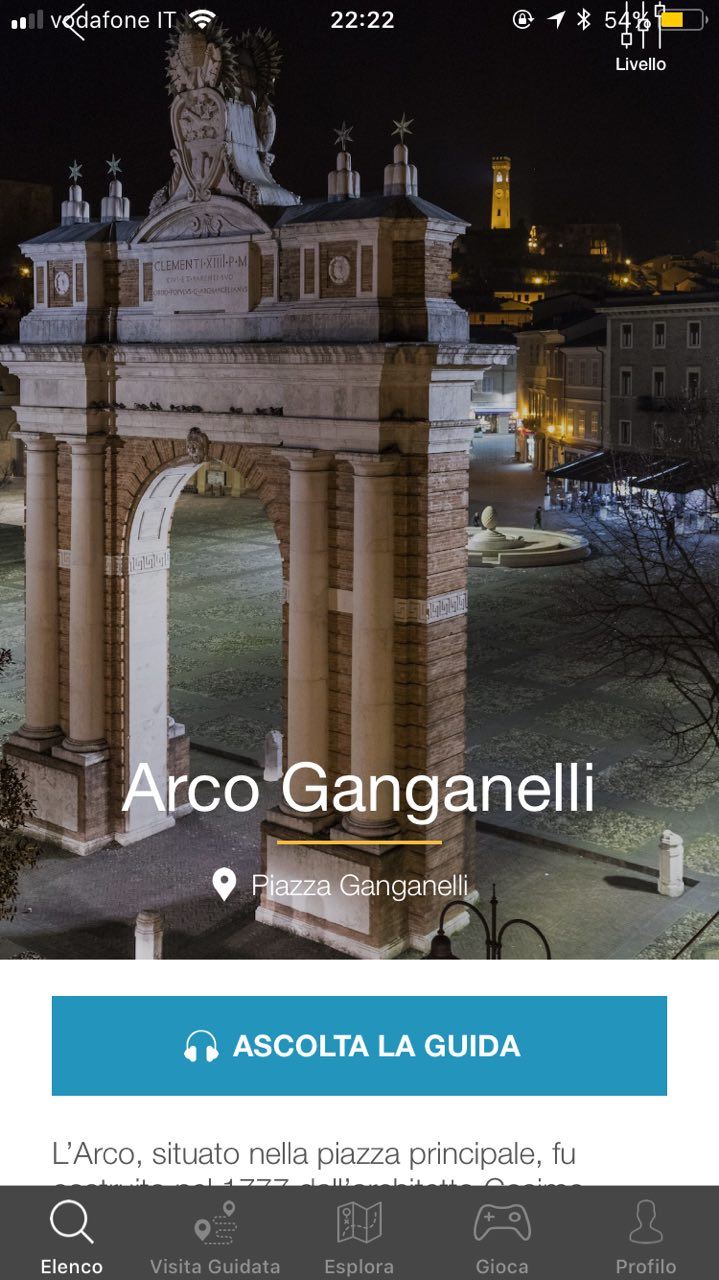
\includegraphics[width=0.3\textwidth]{images/screenSantarcangelo1.jpg}
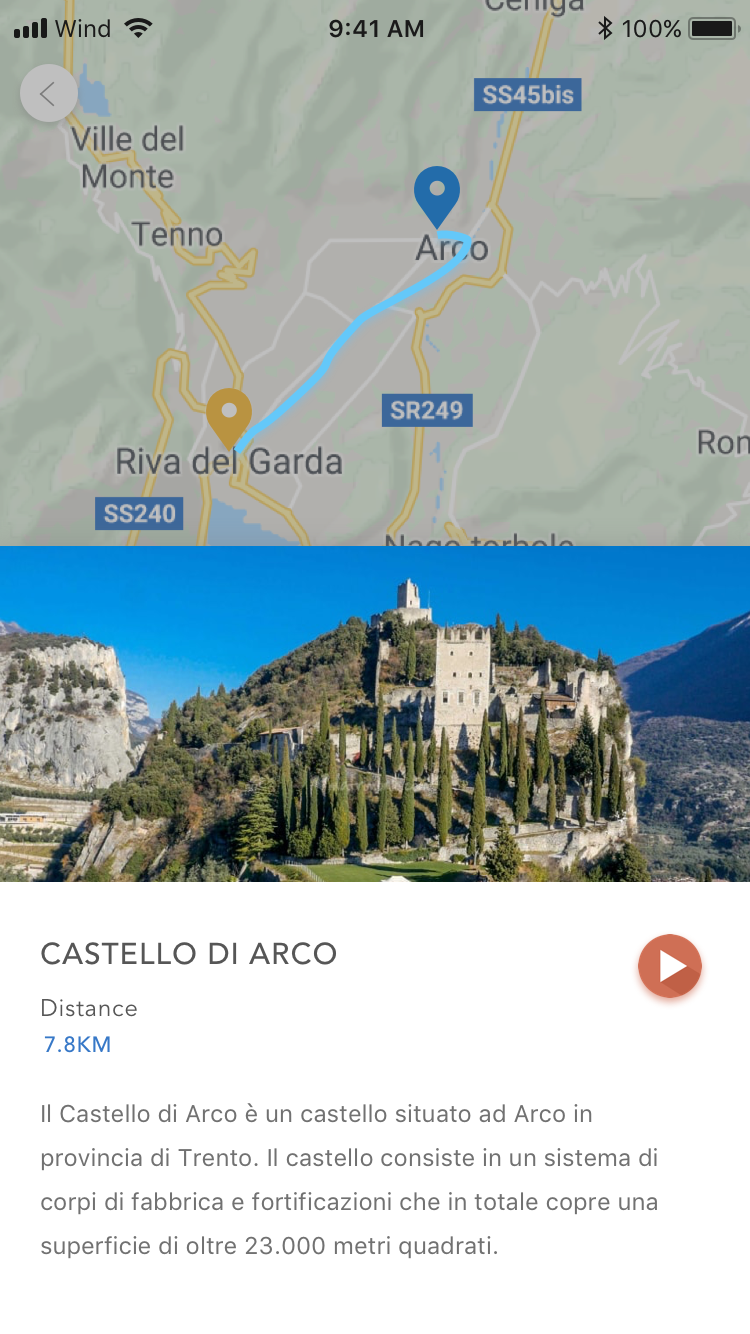
\includegraphics[width=0.3\textwidth]{images/singolopunto.png}
\caption{Confronto HomeScreen Open Air Museum vecchia e nuova versione}
\end{figure}
\vspace{5mm}

\begin{figure}[h]
\centering
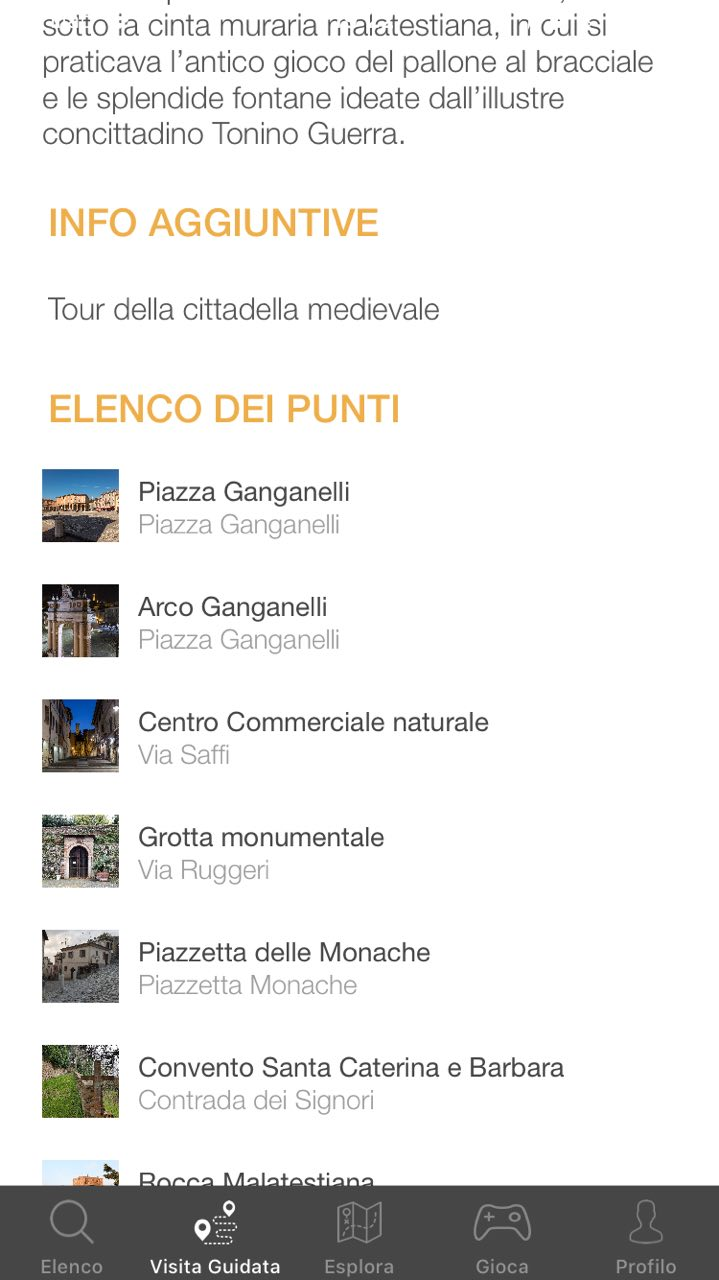
\includegraphics[width=0.3\textwidth]{images/listapercorsiold.jpg}
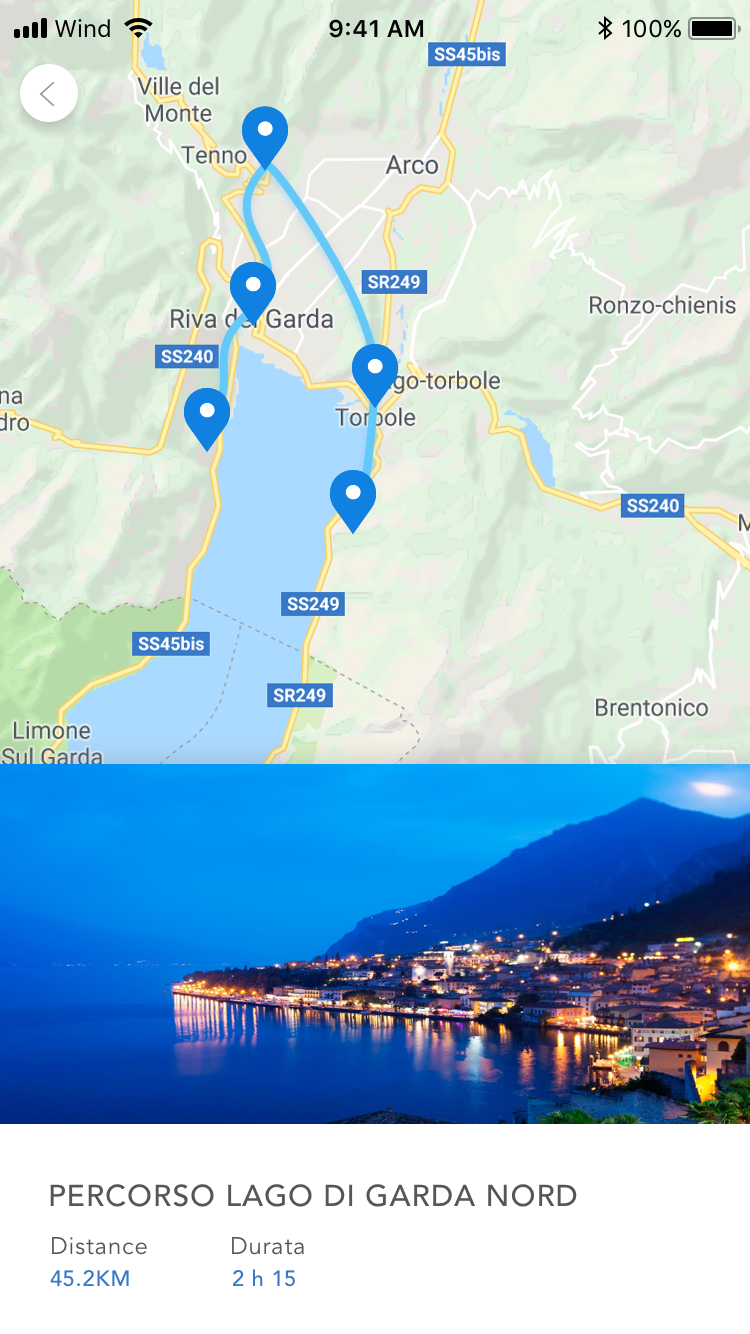
\includegraphics[width=0.3\textwidth]{images/listapercorsi.png}
\caption{Confronto HomeScreen Open Air Museum vecchia e nuova versione}
\end{figure}
\vspace{5mm}


Sfruttando la potente libreria di animazioni fornite da React-native è stato possibile creare un'interfaccia ricca e moderna mantenendo le prestazioni elevate anche su dispositivi non recenti e di alta fascia. Il “driver” di tale libreria è infatti nativo ed implementato nel modo più efficiente per i due sistemi operativi. Questo offre solide prestazioni anche nel caso di animazioni molto complesse ma aggiunge anche alcune limitazioni. La più evidente è l’obbligo di implementare tali animazioni con un pattern dichiarativo indicando quindi in precedenza il modo in cui l’oggetto deve comportarsi per poi avere la possibilità di eseguirlo mediante un'interfaccia di start e stop. Tale problematica non ha composto un grave problema implementativo. DI fatto si è trattato solamente di implementare il tutto seguendo il pattern descritto sopra.\vspace{5mm}

Un'ulteriore funzionalità richiesta al porting è quella di poter, riprodurre dei contenuti audio all’interno dell’applicativo. In particolare questi contenuti audio sono presenti sul server e sono serviti attraverso un'api che permette il loro streaming. In precedenza era stato sviluppato un player che utilizzava i rispettivi sdk nativi per controllare l’audio, erano in grado di avviare e stoppare l’audio e proseguire avanti veloce mediante una barra di trascinamento. Le funzionalità per i due sistemi operativi erano le stesse ma viste le diversità tra le due piattaforme è stato necessario re implementare la stessa logica due volte. Utilizzando React-native è stato possibile scrivere la logica una sola volta e condividerla tra le due piattaforme utilizzando un package open source chiamato react-native-audio-streamer. Tale package permette di configurare uno stream audio mediante un url e di controllare la riproduzione, tale libreria utilizza la medesima implementazione attraverso il “bridge” sfruttando a livello nativo due librerie distinte. Per Ios DuoAudioStreamer mentre per Android ExoPlayer. L’utilizzo di tale package accelera lo sviluppo di questa parte mostrando il vantaggio di React-native sopra a soluzioni simili e cioè l’ecosistema. Creare una dipendenza esterna in un progetto enterprise come questo può essere una scelta rischiosa. Legarsi ad un software di terze parti per una features cruciale dell’applicativo può sfociare in problematiche che spaziano dal mantenimento futuro a bug non facilmente tracciabili ma data la semplicità di questa particolare libreria tale rischio è ragionevolmente contenuto.\vspace{5mm}

Come si è visto l’impiego di React-native non ha soppiantato la totalità della parte nativa, anzi questo approccio “misto” ha permesso di non trovarsi limitati da una tecnologia rispetto ad un altra offrendo sempre il giusto tool per la features richiesta. Durante le ricerche legate allo sviluppo di questo prodotto non sono stati trovati linguaggi o framework più flessibili e adatti alle molteplici configurazioni di questo progetto, questo specifico caso è un ottimo esempio di come l’impiego di Javascript al di fuori dal browser sia la scelta vincente per creare un applicativo moderno e flessibile senza sacrificare manutenibilità e consistenza nel tempo.\vspace{5mm}

\section{Punti critici e problematiche}
\vspace{5mm}Durante questo porting sono stati evidenziati una serie di punti critici implementativi, ne discuterò indicando la soluzione da me intrapresa e se presente una soluzione alternativa.\vspace{5mm}

L’utilizzo di una libreria esterna come quella per la gestione degli stream audio oppure quella per gestire la mappa, creano delle dipendenze che aggiungono una serie di incognite sulla longevità del prodotto. E’ importante legare il progetto il meno possibile a risorse esterne non del tutto affidabili. Per tale ragione entrambe le risorse esterne che l’applicativo utilizza e cioè la libreria per lo streaming audio e l’SDK Estimote sono gestite attraverso un layer software. L’applicativo utilizza la libreria attraverso le Api fornite da questa interfaccia, in caso di necessità si può sostituire più agevolmente la vecchia libreria con la nuova mappando le nuove api sull’interfaccia. Ovviamente questo è possibile nei limiti di una coesione logica tra la il vecchio e nuovo SDK. Da notare che un'implementazione di questo tipo permette inoltre di abbandonare del tutto il software esterno implementando la propria libreria integrandola nel progetto facilmente attraverso tale interfaccia. Un ulteriore possibile soluzione a questo problema sarebbe quello di gestire internamente la maggior parte del software ma in alcuni casi questa soluzione deve essere scartata per l’elevato costo.\vspace{5mm}

Altra problematica è data dalla coesistenza di tre linguaggi differenti nella stessa codebase. In alcuni casi React-native può aggiungere complessità invece che rimuoverla, infatti se la quantità di codice nativo a cui dover attingere è molto grande si rischia di dover mantenere tre ecosistemi a differenza di due. Maggiori sono le tecnologie da conoscere per operare su di un prodotto maggiore è il bagaglio necessario per mantenerlo, questo rende il software più complesso da gestire. In questo caso un'attenta analisi del progetto prima dello sviluppo può guidare verso una soluzione differente ed evitare il problema. Nel caso specifico la quantità di codice nativo necessaria non è stata molta ma tale problema potrà presentarsi in futuro con il proseguire del progetto.\vspace{5mm}

Un alto punto critico da mantenere in considerazione con questo tipo di porting è la completa scomparse di database Sql in favore di uno state manager ad oggetti. Data l'impossibilità di gestire i dati in modo paritetico rispetto alla versione nativa è stato necessario riadattare la logica applicativa a questa nuova tecnologia. Non esistendo più tempi di latenza per accedere ai dati questo ha migliorato molto la pulizia e l'asciuttezza del codice. La modifica dei dati avviene attraverso mutazioni allo stato e questo comporta in caso di applicativi molto grandi una crescente complessità se non si dividono in modo accorto le varie aree dello stato dividendo in modo netto una area dall'altra usando nodi il più possibile vicini alla radice. Tale approccio infatti permette di ottenere una buona "separation of concerns"\cite{SOC} delle varie aree logiche dell'applicativo ponendo entrypoint diversi per l'accesso ai dati a seconda della zona logica prestabilita. Ciò permette di risolvere il problema descritto sopra, offrendo un guadagno in termini di semplicità rispetto ad una soluzione basata su SqLite.


      \chapter{Applicazioni future}
\label{cha:intro}
\vspace{5mm}

Uno degli aspetti principali che hanno portato al refactor di questo progetto è stata quella di renderlo più flessibile ed adattabile ad altri contesti e non solo legato al comune che ha commissionato l’applicativo. Un ulteriore passo in questa direzione è lo sviluppo di un altro applicativo che abbia le funzionalità di un orchestratore. Tale applicativo, anch'esso sviluppato mediante Nodejs sarà in grado di sfruttare a pieno l’alta configurabilità di ogni applicativo che comprende lo stack Alakai, eseguendo in modo automatizzato la configurazione e il deploy di tutti i servizi necessari. Per raggiungere tale scopo è necessario implementare alcuni accorgimenti. I punti che descriverò ora sono delle linee guida generali e non passaggi sequenziali verso un prodotto finito.\vspace{5mm}

Il primo tra questi è possedere un portale dove richiedere all’utente le configurazioni necessarie, come il nome dell’applicativo, se si desidera utilizzare o meno l’Estimote SDK oppure utilizzare il GPS, le Api key di Eventbrite e le chiavi degli store per la firma degli applicativi per IOS e per Android. Una volta ottenute queste informazioni è necessario costruire un manager che, una volta importata la configurazione, esegua un deploy della parte server in Nodejs, trasponga l’applicativo admin in React e lo inserisca all’interno di una directory prestabilita sul server in modo che possa essere servito staticamente e infine compili e firmi i due applicativi per Android e IOS. Le problematiche da risolvere per raggiungere un prodotto di questo tipo sono molteplici, ne discuterò solo alcune.\vspace{5mm}

E’ necessario possedere un ambiente in grado di ospitare un applicativo in Nodejs e servire mediante un proxyPass sia l’applicativo in React sia le Api sullo stesso dominio. Per fare questo è necessario che la macchina abbia installata una versione di Node Js superiore al 6 e aver installato e configurato Nginx o Apache in modo da implementare il proxyPass descritto sopra. Tali configurazioni sono di fatto uguali ad ogni istanza che si desidera allocare per cui una soluzione per gestire ed automatizzare il tutto è utilizzare un'immagine Docker. Docker permette di creare delle istanze, chiamate container, separate dal sistema operativo che le ospita.Tali istanze sono meno pesanti rispetto ad una macchina virtuale, questo grazie alla condivisione delle risorse del kernel tra i vari container. Oltre a ciò sono, grazie alla condivisione delle risorse a basso livello, molto veloci da avviare e da arrestare e questo rende Docker la tecnologia perfetta per questo genere di problematiche.
L’idea è quella di creare un immagine docker che contiene NodeJs e Nginx insieme alla sua configurazione ed iniettare all’interno di essa, al momento della creazione dell’istanza, il codice sorgente configurato mediante i dati inviati dall’utente.\vspace{5mm}

Per quanto riguarda invece la compilazione e la firma degli applicativi mobili è necessario configurare in modo particolare la macchina che eseguirà questo tipo di task. Di fatto bisogna che sia una versione di macOs visto che Apple non fornisce ad ora una versione di XCode per sistemi linux o Windows. Per quanto riguarda Android è necessario installare la command line interface del Gradle. A questo punto sarà necessario preparare uno script in bash che eseguirà una volta chiamato, tutte le procedure di compilazione e di firma degli applicativi. Tale procedura dovrà renderli disponibili al download inserendoli in una apposita directory dove un applicativo gli servirà e potranno essere scaricati e distribuiti attraverso gli store.\vspace{5mm}

Questi sono alcuni dei punti implementativi da svolgere per arrivare ad avere un prodotto con queste features. L’architettura progettuale risultante sarà simile a quella descritta in figura\vspace{5mm}

\begin{figure}[h]
\centering
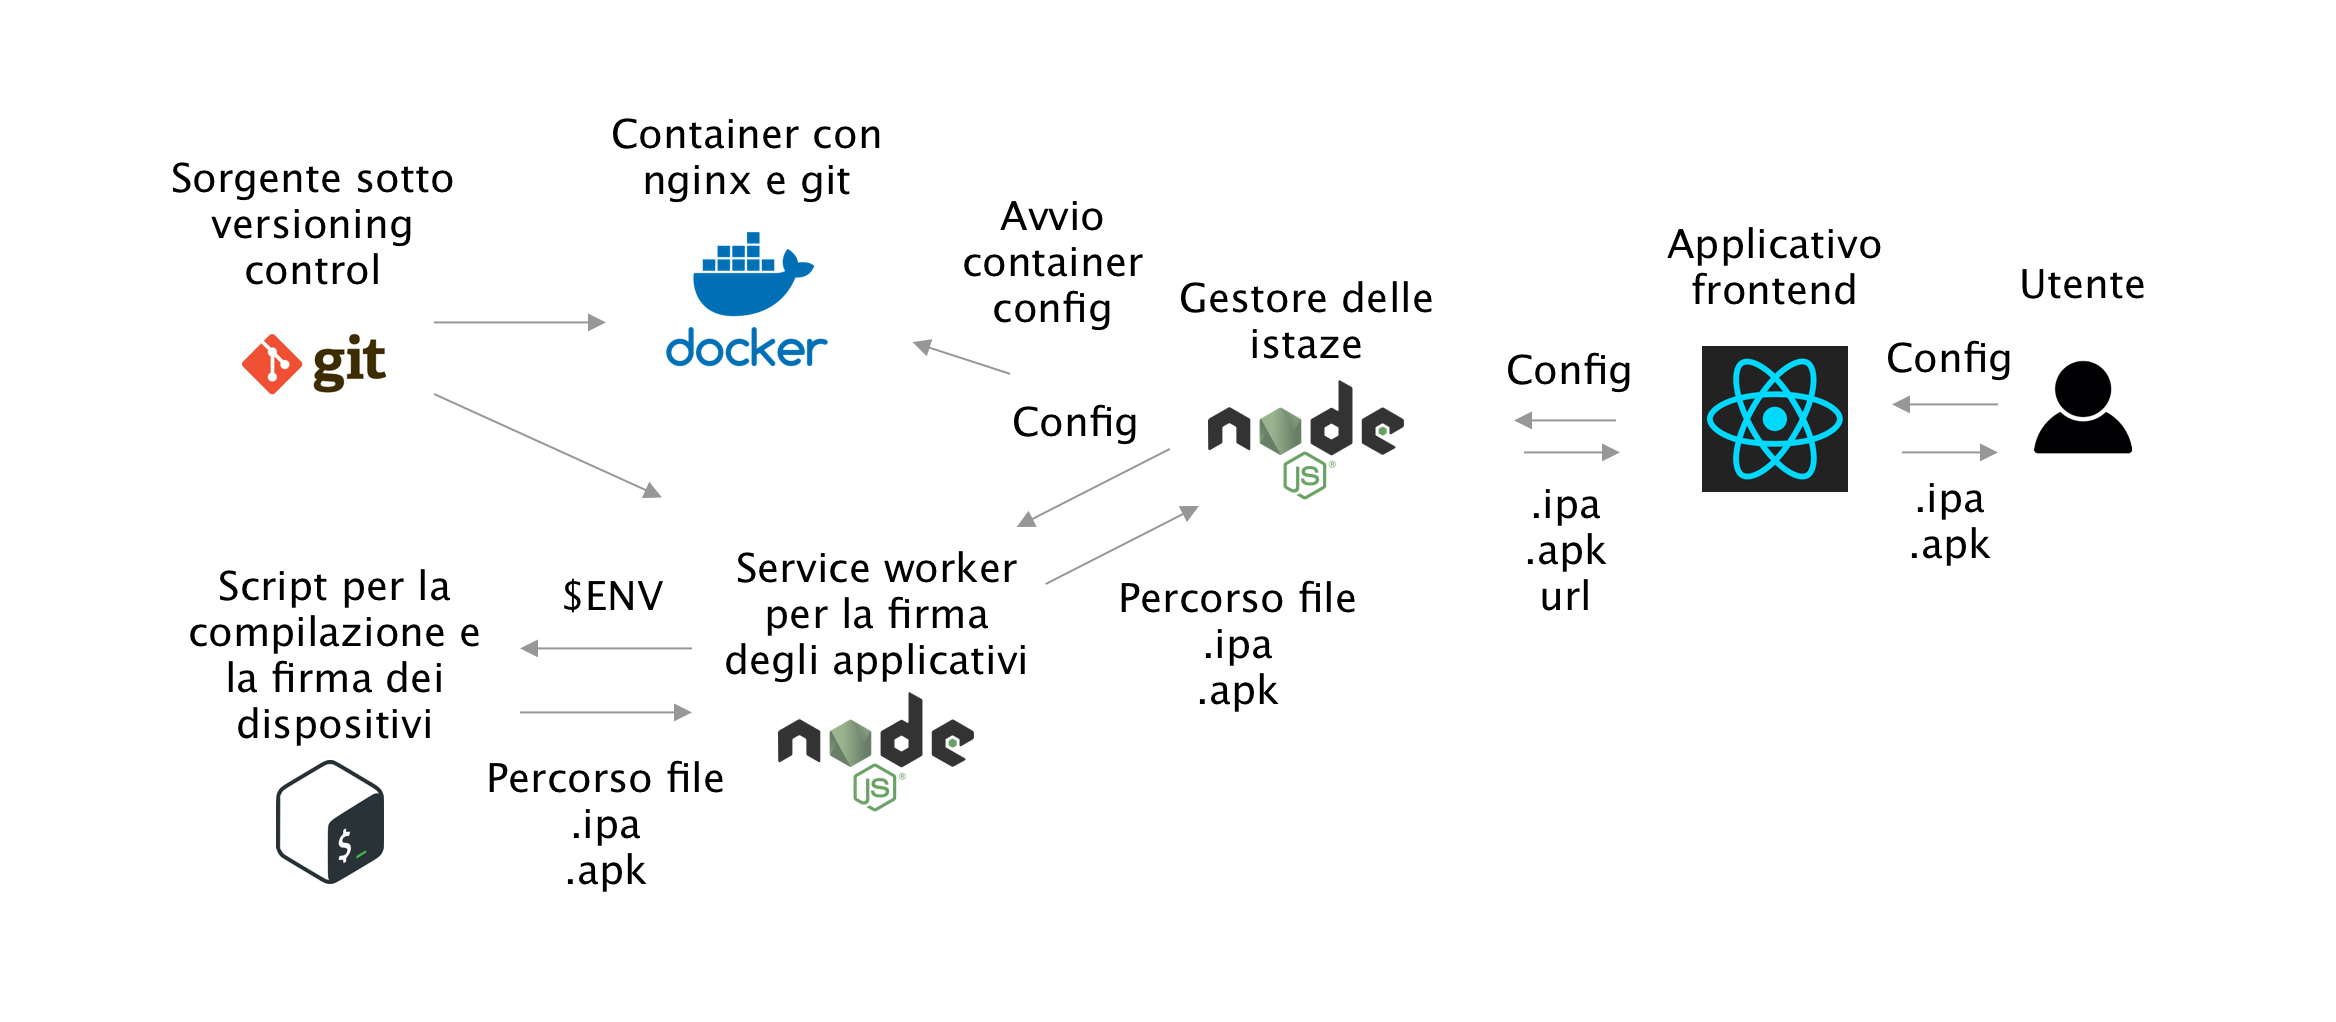
\includegraphics[width=1\textwidth]{images/schemaIstanzeAlakai.png}
\caption{Schema del funzionamento della possibile futura del Control Manager di istanze di Open Air Museum}
\end{figure}

Come si può notare vi sarà un service worker sviluppato in node che controllerà l’esecuzione dello script bash iniettando tutte le variabili di environment come i percorsi ai certificati ,precedentemente caricati, indispensabili per la procedura di compilazione e di firma.\vspace{5mm}

      \chapter{Analisi e Conclusioni}
\label{cha:intro}
\vspace{5mm}

Per discutere di ciò che il refactor ha portato dividerò le conclusioni in due parti prendendo in considerazione prima il lato tecnologico e poi il lato umano. Ponendo che il progetto è in fase di terminazione non vi è la possibilità di accedere a dati definitivi per cui quello che riporterò di seguito potrebbero essere soggetto a variazioni future.\vspace{5mm}

 Previa analisi è necessario fornire un contesto per qualificare al meglio i dati che andrò a descrivere, il primo fattore sono il numero di sviluppatori dedicati a questo progetto. La composizione dell'organico è il seguente, un grafico, due programmatori ed un project manager il quale compito era gestire la qualità del prodotto e far rispettare le tempistiche promesse al cliente.\vspace{5mm}

Prendendo in considerazione il lato umano è subito risultato lampante come, seppur la divisione dei compiti dello sviluppo era fatta per ambienti e cioè lato client e lato server, la facilità con cui il team ha potuto interscambiarsi è stata molto evidente. Si è mostrato come, seppur la codebase fosse nuova e solo la logica generale fosse conosciuta, possedere una 'lingua franca' in cui esprimersi è stato fondamentale per velocizzare tutte quelle operazioni che richiedevano di muoversi in un differente. Un altro esempio di questo è la velocità con cui si sono eseguite le code review settimanali. Possedere un dialetto comune permette di rendere più veloce la comprensione delle features aggiunte dal collega e trovare eventuali bug o problemi in modo più immediato. Ecco che grazie a questo tipo di approccio si è potuto delineare una tecnica di divisione dei compiti non più per zona di lavoro (server o client) ma per funzionalità. Si è notato che la velocità di sviluppo aumentava se, isolata una features, chi aveva il compito di implementarla creava sia il lato client che il lato server. Questo ha evitato anche lo sviluppo di rest api ridondanti con dati mai utilizzati a front end, aumentando l'efficenza del software, evitando di dover eseguire lo step intermedio di accordarsi, per ogni nuova funzionalità che si andava ad inserire, sulla forma delle api. Ora di fatto chi sviluppa la funzionalità lato utente ha anche il compito di sviluppare le api che dovranno essere consumate per fornire tale funzionalità creando un prodotto meno frammentato e più integrato. \vspace{5mm}

Un altro punto focale è stata la possibilità di condividere conoscenze in modo più diretto. Molte delle tecnologie e dei pattern di programmazione utilizzati principalmente a lato client hanno contaminato il lato server e vice versa. Librerie come Redux sono agnostiche e possono adattarsi facilmente al contesto server e pattern come la programmazione funzionale possono essere distribuite senza difficoltà nell'intera codebase del progetto evitando "l'effetto palude". Tale effetto è quando durante lo sviluppo una parte di codice non mantenuta diventa ingestibile a causa dell'incapacità dei colleghi di fare refactor su quella parte perché scritta con un certo linguaggio non conosciuto da tutti i componenti del team, o con un pattern conosciuto solamente dal suo scrittore. Con uno stack full Javascript come quello proposto nella soluzione descritta in questa tesi si può risolvere senza overhead questo genere di problemi forzando un vero standard in tutta la code base superando i limiti tecnologici imposti da un cambio di linguaggio tra due aree.\vspace{5mm}

Ulteriore appunto che è emerso durante lo sviluppo è stata la possibilità di condividere alcune logiche tra client e server, tagliando notevolmente i tempi di sviluppo. Tutte le logiche per il recupero dei dati sono state racchiuse in una piccola libreria che è stata condivisa tra gli applicativi mobili e il lato admin. La scrittura di un solo pezzo di codice destinato ad uno scopo preciso e portabile su più piattaforme ha inoltre evitato bug derivati da modifiche alle api dato che per più volte è bastato aggiornare internamente la libreria senza dover cambiare null'altro.\vspace{5mm}

Un ultimo punto che voglio includere che non è legato ad una situazione generica ma solamente al mio ambiente lavorativo; essendo Farnedi ICT in primis un azienda che fa supporto tecnico ad aziende e p.a. parte dei suoi dipendenti non hanno una conoscenza diretta di sviluppo software. Javascript è risultato essere molto chiaro anche a chi è al di fuori del campo, permettendo anche al lato manageriale di entrare, in minima parte, nello sviluppo. Tale considerazione potrebbe essere legata alla mia sola realtà aziendale ma è stata di grande importanza per la produzione di funzionalità qualitativamente più in linea con le richieste del direttivo.\vspace{5mm}

Dal punto di vista tecnologico non vi sono stati cambiamenti importanti, le funzionalità applicative trattandosi di un refactor hanno seguito la linea del prodotto iniziale. Però la dismessa di un applicativo come filemaker per il recupero dei dati è stata la fonte di un incremento sostanziale nella mantenibilità e nella rapidità dell'applicativo in tutte le sue parti. La scelta di passare da un applicativo sviluppato con un framework proprietario ad un tool open source come React ha portato in generale ad ottenere un ambente di sviluppo più moderno e flessibile. Il passaggio ad una SPA\cite{SPA} ha migliorato non solo l'esperienza per chi ha sviluppato il software ma la qualità del prodotto in se.\vspace{5mm}

Per quanto riguarda i costi di refactor degli applicativi è risultato in un consumo di ore uomo differente a seconda dell'ambito del refactor. Nel caso dell'applicativo admin lo sviluppo è stato più costoso in ore lavoro rispetto alla versione precedente in Filemaker ma, ciò ha tolto ulteriore lavoro necessario per adattare i dati provenienti da filemaker alla struttura del database. Per quanto riguarda invece lo sviluppo degli applicativi mobili React-native ha portato un enorme vantaggio riducendo alle versioni divise, infatti lo sviluppo necessario per il completaemnto di entrambe le versioni è stato un terzo rispetto al precedente.\vspace{5mm}  

\section{Confronto tra le due versioni}\vspace{5mm}  

Confrontando gli stack delle due applicazioni in termini di tecnologie utilizzate possiamo vedere i motivi per cui le scelte fatte migliorano il software e sotto quali aspetti. \vspace{5mm}

Grazie all'utilizzo del medesimo framework lato mobile e lato web è stato possibile condividere gran parte del codice e delle logiche di interazione con le api lato server. Un altra zona di condivisione è l'implementazione di Redux. Data la sua agnosticità sulla piattaforma utilizzata questa libreria è un perfetto esempio di come l'utilizzo di uno stack basato interamente su Javascript porti ad un riutilizzo del codice in modo importante ma sopratutto in modi impraticabili precedentemente. In particolare tra l’applicativo admin sviluppato come webapp per il browser e gli applicativi nativi ho condiviso la totalità dell’implementazione gestendo lo store allo stesso modo. Le differenze principali sono sulla libreria che permette di interfacciarsi con le api lato server. Seppur molti metodi sono condivisi, quelli relativi alla mutazione dei dati sono riserveti ai soli utenti autenticati e cioè Admin. Tale peculiarità però non influisce nella possibilità di riutilizzare parte della libreria che implementa sia i metodi lato amministratore che quelli lato utente senza privilegi.\vspace{5mm} 

Un ulteriore punto è che rispetto alla versione precedente vi è una somiglianza molto forte tra quello che è l’applicativo web e l’applicativo nativo, le due applicazioni non sono compatibili ma condividono gran parte delle logiche e dei pattern essendo di fatto lo stesso framework. Ciò permette di avere un livello di complessità all'approccio a questo progetto più bassa della versione precedente. Questo porta a tempi più corti per l'apprendimento dei pattern e delle logiche e di conseguenza risulta in una miglior produttività.\vspace{5mm}
	
La scelta dell’utilizzo di un database a file con la possibilità di configurare e passare ad un database “classico” si è rivelata molto importante per la scalabilità dell’applicativo. SqLite risulta più comodo in fase di deploy di contro, non ha le prestazioni di un database “classico” e la possibilità di configurare rapidamente la tecnologia da utilizzare è un plus importante. Questo si ottiene grazie all’impiego di un ORM in grado di fornire questa features come Sequelize. Oltre a questo permette di implementare in modo veloce migrazioni e seeder restando sempre agnostico sulla tecnologia a database. La versione precedente conteneva una pesante assunzione sull’utilizzo di un database MySql e ciò abbassava sostanzialmente la flessibilità e il riutilizzo del prodotto.\vspace{5mm}

Un altra differenza rispetto alla precedente è l’esistenza dell’applicativo admin in react che dovrà essere servito dall’applicativo server. Per fare questo è necessario che tutte le richieste non inviate direttamente a /api, vengano tutte reindirizzare all’applicativo in modo che la SPA utilizzi il router interno a React per mostrare i contenuti corrispondenti all’url della richiesta.\vspace{5mm}

Riguardo al lato “admin”, cioè quello che va a sostituire Filemaker nella raccolta dati, è stato sviluppato con React. La scelta di sviluppare una SPA\cite{SPA} per questo compito è stata dettata da un bisogno di rendere questa operazione iterabile e ripetibile. Nel caso in cui il cliente volesse cambiare dei testi o correggere delle traduzioni può farlo in autonomia, senza dover passare da una figura che traduca le modifiche richieste aggiungendole a database manualmente. Questo processo inoltre astrae ulteriormente la struttura del database durante il processo di inserimento dei dati offrendo quindi flessibilità su modifiche future alla struttura. Un altro punto a favore della scelta di una SPA \vspace{5mm}

\section{Punti critici}
\vspace{5mm}L'utilizzo di una sola tecnologia in più zone distinte dello stack porta con se numerosi vantaggi che ho descritto precedentemente. Va detto però che se nello specifico caso applicativo preso da me come esempio le tecnologie Javascript esistenti sul mercato andavano a completare in modo ottimale le necessità applicative, questo può non essere vero per tutti i casi. In linea generale è sempre meglio scegliere la tecnologia migliore per la funzionalità che si vuole svolgere. Un esempio è la capacità computazionale limitata di Javascript che a confronto con Python non permette di svolgere in modo efficiente operazioni su matrici limitandone l'uso per quanto riguarda l'ambito del machine learning. In questo caso Javascript potrebbe far eseguire le operazioni di calcolo sfruttando l'ambiente fornito da Node e in particolare eseguire dei processi stando in ascolto di essi, in attesa di risultati sfruttando l'asicronicità dell'I/O fornita dal framework. Tali processi, disegnati per eseguire micro task di computazione matematica, potrebbero essere sviluppati in c o c++ in modo da essere il più ottimizzati possibile per il compito. Tale approccio però offre il fianco ad una serie di problematiche legate alla mantenibilità della parte in c++ e alla dipendenza non diretta del software Javascript a tale libreria. Per avere questo tipo di dipendenza è necessario crearla attraverso una struttura software per interrompere l'esecuzione o mostrare degli errori all'avvio in caso tali dipendenze non siano esplicitate.

\vspace{5mm}La scelta di utilizzare un database a file per conservare i dati sui vari punti rende problematico scalare il prodotto. Infatti, nel caso si voglia far pilotare questo applicativo da un loadbalancer\cite{LoadBalancing} in grado di animare istanze a seconda del carico, ogni istanza non sarà in grado di condividere dati tra di essa creando un grave problema di consistenza. Per questa ragione la scelta di utilizzare questo tipo di tecnologia è fallimentare in quest'ottica. Una soluzione per dare la possibilità di scalare all'applicativo è quella di sfruttare la flessibilità di Sequelize\cite{Sequelize} che permette di mantenere la stessa struttura dei modelli ma di cambiare la tecnologia del database. E' grazie a questa astrazione software che si è in grado di adattare il nuovo applicativo ad altri contesti di utilizzo.










      %\input{capitolo4}
      
      
    \endgroup


    % bibliografia in formato bibtex
    %
    % aggiunta del capitolo nell'indice
    \addcontentsline{toc}{chapter}{Bibliografia}
    % stile con ordinamento alfabetico in funzione degli autori
    \bibliographystyle{plain}
    \bibliography{biblio}
%%%%%%%%%%%%%%%%%%%%%%%%%%%%%%%%%%%%%%%%%%%%%%%%%%%%%%%%%%%%%%%%%%%%%%%%%%
%%%%%%%%%%%%%%%%%%%%%%%%%%%%%%%%%%%%%%%%%%%%%%%%%%%%%%%%%%%%%%%%%%%%%%%%%%
%% Nota
%%%%%%%%%%%%%%%%%%%%%%%%%%%%%%%%%%%%%%%%%%%%%%%%%%%%%%%%%%%%%%%%%%%%%%%%%%
%% Nella bibliografia devono essere riportati tutte le fonti consultate 
%% per lo svolgimento della tesi. La bibliografia deve essere redatta 
%% in ordine alfabetico sul cognome del primo autore. 
%% 
%% La forma della citazione bibliografica va inserita secondo la fonte utilizzata:
%% 
%% LIBRI
%% Cognome e iniziale del nome autore/autori, la data di edizione, titolo, casa editrice, eventuale numero dell’edizione. 
%% 
%% ARTICOLI DI RIVISTA
%% Cognome e iniziale del nome autore/autori, titolo articolo, titolo rivista, volume, numero, numero di pagine.
%% 
%% ARTICOLI DI CONFERENZA
%% Cognome e iniziale del nome autore/autori (anno), titolo articolo, titolo conferenza, luogo della conferenza (città e paese), date della conferenza, numero di pagine. 
%% 
%% SITOGRAFIA
%% La sitografia contiene un elenco di indirizzi Web consultati e disposti in ordine alfabetico. 
%% E’ necessario:
%%   Copiare la URL (l’indirizzo web) specifica della pagina consultata
%%   Se disponibile, indicare il cognome e nome dell’autore, il titolo ed eventuale sottotitolo del testo
%%   Se disponibile, inserire la data di ultima consultazione della risorsa (gg/mm/aaaa).    
%%%%%%%%%%%%%%%%%%%%%%%%%%%%%%%%%%%%%%%%%%%%%%%%%%%%%%%%%%%%%%%%%%%%%%%%%%
%%%%%%%%%%%%%%%%%%%%%%%%%%%%%%%%%%%%%%%%%%%%%%%%%%%%%%%%%%%%%%%%%%%%%%%%%%
    

    \titleformat{\chapter}
        {\normalfont\Huge\bfseries}{Allegato \thechapter}{1em}{}
    % sezione Allegati - opzionale
    \appendix
    \chapter{Schemi ER}

\begin{figure}[h]
\centering
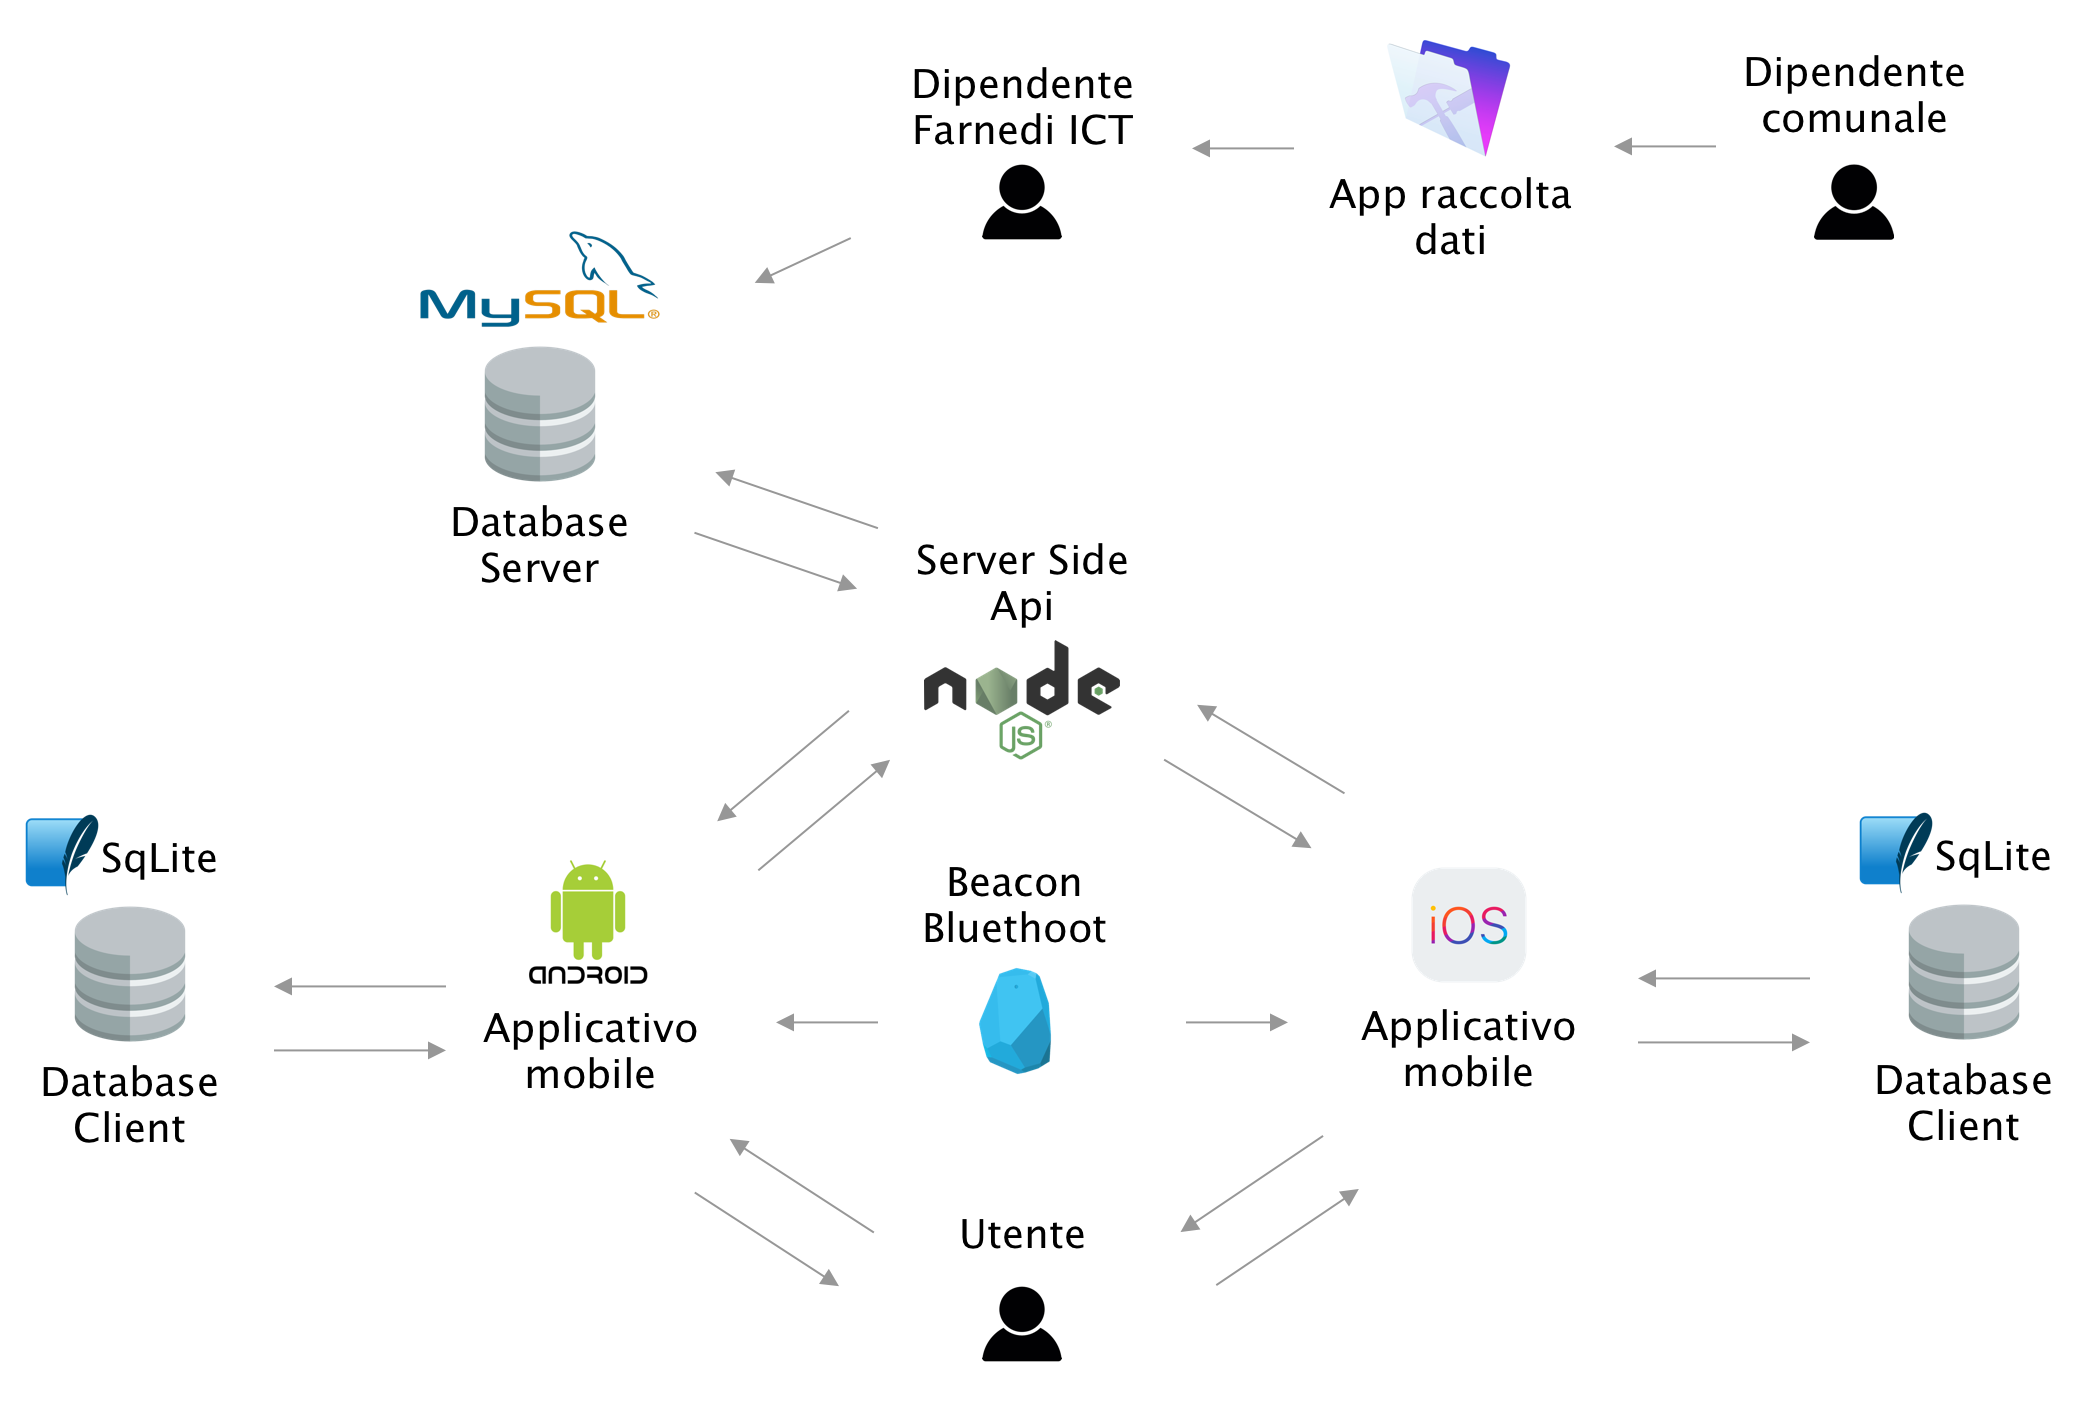
\includegraphics[width=0.6\textwidth]{images/SchemaOpenAirMuseum.png}
\caption{Schema ER dell'applicativo server}
\end{figure}
				
\begin{figure}[h]
\centering
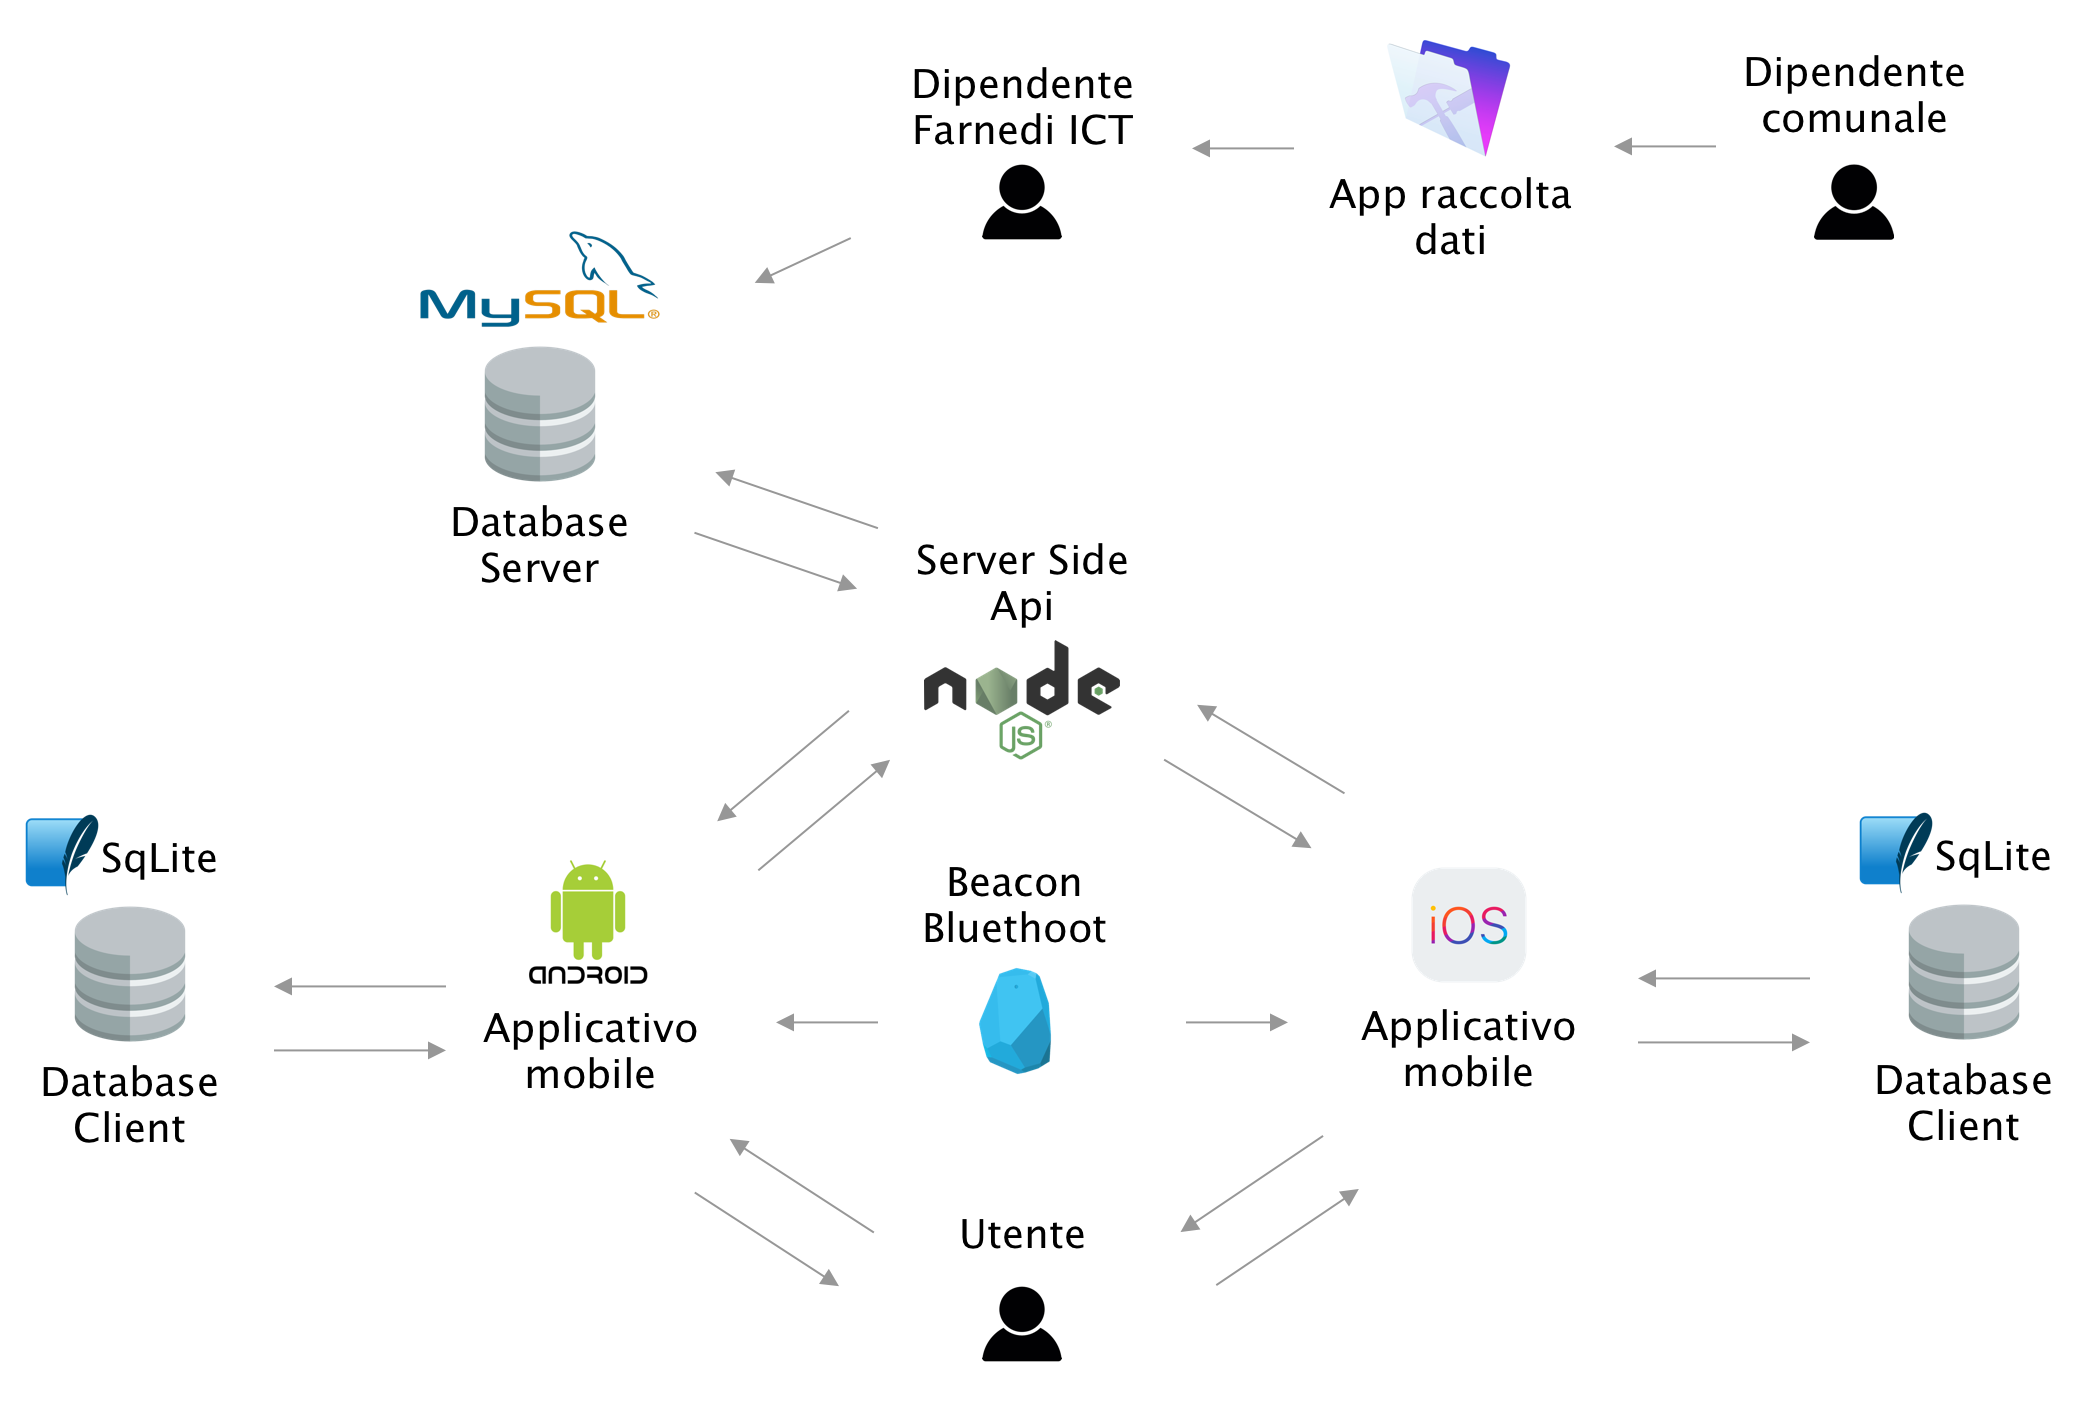
\includegraphics[width=0.6\textwidth]{images/SchemaOpenAirMuseum.png}
\caption{Schema ER degli applicativi mobili}
\end{figure}


\end{document}
